\documentclass[semifinal]{cpecmu}

%% This is a sample document demonstrating how to use the CPECMU
%% project template. If you are having trouble, see "cpecmu.pdf" for
%% documentation.

% \projectNo{P069-1}
% \acadyear{2021}

\titleTH{รายงานสหกิจศึกษาตําแหน่ง Fullstack Deverloper ที่ G-ABLE}
\titleEN{Cooperative Education Report for the Position of Fullstack Developer at G-ABLE}

\author{นายสิปปกร คำมีสว่าง}{Sippakon Khammisawang}{650610813}
% \author{นายบรรจบ พบเอฟตลอด}{Banjob Pob-eftalord}{690610969}

\cpeadvisor{chinawat}
\cpecommittee{paskorn}
% \committee{รศ.ดร.\,นิพนธ์ ธีรอำพน}{Assoc.\,Prof.\,Nipon Theera-Umpon, Ph.D.}

%% Some possible packages to include:
\usepackage[final]{graphicx} % for including graphics

%% Add bookmarks and hyperlinks in the document.
\PassOptionsToPackage{hyphens}{url}
\usepackage[colorlinks=true,allcolors=Blue4,citecolor=red,linktoc=all]{hyperref}
\def\UrlLeft#1\UrlRight{$#1$}

%% Needed just by this example, but maybe not by most reports
\usepackage{afterpage} % for outputting
\usepackage{pdflscape} % for landscape figures and tables. 
\usepackage{minted}
\usepackage{pdfpages}
\usepackage{hyperref}
\usepackage{pdfpages}
\usepackage{fancyhdr}
\usepackage{import}
\usepackage{longtable}
\usepackage{array}
\usepackage{tabularx}
\usepackage{etoolbox}
\usepackage{changepage}
\usepackage{mdframed}

%% Some other useful packages. Look these up to find out how to use
%% them.
% \usepackage{natbib}    % for author-year citation styles
% \usepackage{txfonts}
% \usepackage{appendix}  % for appendices on a per-chapter basis
% \usepackage{xtab}      % for tables that go over multiple pages
% \usepackage{subfigure} % for subfigures within a figure
% \usepackage{pstricks,pdftricks} % for access to special PostScript and PDF commands
% \usepackage{nomencl}   % if you have a list of abbreviations

%% if you're having problems with overfull boxes, you may need to increase
%% the tolerance to 9999
% \tolerance=9999

\bibliographystyle{plain}
% \bibliographystyle{IEEEbib}

% \renewcommand{\topfraction}{0.85}
% \renewcommand{\textfraction}{0.1}
% \renewcommand{\floatpagefraction}{0.75}

%% Example for glossary entry
%% Need to use glossary option
%% See glossaries package for complete documentation.
\ifglossary
  \newglossaryentry{lorem ipsum}{
    name=lorem ipsum,
    description={derived from Latin dolorem ipsum, translated as ``pain itself''}
  }
\fi

%% Uncomment this command to preview only specified LaTeX file(s)
%% imported with \include command below.
%% Any other file imported via \include but not specified here will not
%% be previewed.
%% Useful if your report is large, as you might not want to build
%% the entire file when editing a certain part of your report.
% \includeonly{chapters/intro,chapters/background}

\begin{document}
\maketitle
\makesignature

\ifproject
\begin{abstractTH}
% เขียนบทคัดย่อของรายงานที่นี่

% การเขียนรายงานเป็นส่วนหนึ่งของการทำรายงานวิศวกรรมคอมพิวเตอร์
% เพื่อทบทวนทฤษฎีที่เกี่ยวข้อง อธิบายขั้นตอนวิธีแก้ปัญหาเชิงวิศวกรรม และวิเคราะห์และสรุปผลการทดลองอุปกรณ์และระบบต่างๆ
% \enskip อย่างไรก็ดี การสร้างรูปเล่มรายงานให้ถูกรูปแบบนั้นเป็นขั้นตอนที่ยุ่งยาก
% แม้ว่าจะมีต้นแบบสำหรับใช้ในโปรแกรม Microsoft Word แล้วก็ตาม
% แต่นักศึกษาส่วนใหญ่ยังคงค้นพบว่าการใช้งานมีความซับซ้อน และเกิดความผิดพลาดในการจัดรูปแบบ กำหนดเลขหัวข้อ และสร้างสารบัญอยู่
% \enskip ภาควิชาวิศวกรรมคอมพิวเตอร์จึงได้จัดทำต้นแบบรูปเล่มรายงานโดยใช้ระบบจัดเตรียมเอกสาร
% \LaTeX{} เพื่อช่วยให้นักศึกษาเขียนรายงานได้อย่างสะดวกและรวดเร็วมากยิ่งขึ้น

รายงานฉบับนี้เป็นการนำเสนอผลการปฏิบัติงานสหกิจศึกษาของนักศึกษาวิศวกรรมศาสตรบัณฑิต สาขาวิศวกรรมคอมพิวเตอร์ ในตำแหน่ง Fullstack Developer ที่บริษัท จีเอเบิล จำกัด (G-ABLE Company Limited)
ในระหว่างระยะเวลาการปฏิบัติงาน นักศึกษาได้มีส่วนร่วมในกระบวนการพัฒนาซอฟต์แวร์ทั้งในส่วนของ Frontend และ Backend
โดยมีหน้าที่หลักในการพัฒนาและดูแลระบบเว็บแอปพลิเคชัน ออกแบบและพัฒนา API สำหรับการสื่อสารข้อมูลระหว่างระบบ 
รวมถึงการเชื่อมต่อและจัดการฐานข้อมูลเพื่อให้การทำงานของระบบเป็นไปอย่างมีประสิทธิภาพ 
ซึ่งประสบการณ์ทั้งหมดนี้มีส่วนสำคัญในการเพิ่มประสิทธิภาพและความยืดหยุ่นของกระบวนการพัฒนาซอฟต์แวร์ 
เพื่อให้บริษัทสามารถส่งมอบโซลูชันดิจิทัลที่มีคุณภาพและตอบสนองความต้องการของลูกค้าได้อย่างรวดเร็วและมีประสิทธิผล
\end{abstractTH}

\begin{abstract}
    This report presents the results of the cooperative education experience of a Bachelor of Engineering student in Computer Engineering, who served as a Fullstack Developer at G-ABLE Company Limited.
During the internship period, the student participated in the software development process for both frontend and backend systems. The main responsibilities included developing and maintaining web applications, designing and implementing APIs for data communication between systems, as well as connecting and managing databases to ensure efficient system performance.
All of these experiences played an important role in enhancing the efficiency and flexibility of the software development process, enabling the company to deliver high-quality digital solutions that effectively and promptly meet customer needs.

% Make sure your abstract sits inside the \texttt{abstract} environment.
\end{abstract}

\iffalse
\begin{dedication}
This document is dedicated to all Chiang Mai University students.

Dedication page is optional.
\end{dedication}
\fi % \iffalse

\begin{acknowledgments}
    การที่ข้าพเจ้าได้มาปฏิบัติงานสหกิจศึกษา ณ บริษัท จีเอเบิล จำกัด (มหาชน)  ตั้งแต่วันที่ 16 เมษายน 2568  ถึง วันที่  15 ตุลาคม 2568  ส่งผลให้ข้าพเจ้าได้รับความรู้และประสบการณ์ต่างๆ ที่มีค่ามากมาย สำหรับรายงานวิชาสหกิจศึกษาฉบับนี้  สำเร็จลงได้ด้วยดีจากความร่วมมือและสนับสนุนจากหลายฝ่าย  ดังนี้
    \begin{enumerate}
        \item ปรีชา ปิติจรูญพงศ์ — Lending Business Solution Manager
        \item ไชยา แสงจันทร์ — System Analyst
    \end{enumerate}
    และบุคคลท่านอื่นๆที่ไม่ได้กล่าวนามทุกท่านที่ได้ให้คำแนะนำช่วยเหลือในการจัดทำรายงาน
	ข้าพเจ้าใคร่ขอขอบพระคุณผู้ที่มีส่วนเกี่ยวข้องทุกท่าน ที่มีส่วนร่วมในการให้ข้อมูล เป็นที่ปรึกษาในการทำรายงานฉบับนี้จนเสร็จสมบูรณ์ ตลอดจนให้การดูแลและให้ความเข้าใจเกี่ยวกับชีวิตของการทำงานจริง ข้าพเจ้าขอขอบคุณ ไว้ ณ ที่นี้
    \acksign{2025}{10}{15}
\end{acknowledgments}%
\fi % \ifproject

\contentspage

\ifproject
\figurelistpage

\tablelistpage
\fi % \ifproject

% \abbrlist % this page is optional

% \symlist % this page is optional

% \preface % this section is optional


\pagestyle{empty}\cleardoublepage
\normalspacing \setcounter{page}{1} \pagenumbering{arabic} \pagestyle{cpecmu}

\chapter{\ifenglish Introduction\else บทนำ\fi}

\section{\ifenglish Objectives\else วัตถุประสงค์\fi}
\begin{enumerate}
    \item เพื่อนำความรู้ทั้ง Frontend (การพัฒนาหน้าบ้าน) และ Backend (การพัฒนาหลังบ้าน/ฐานข้อมูล) มาพัฒนาโปรเจกต์หรือระบบจริงขององค์กร
    \item เพื่อฝึกฝนการใช้งานเครื่องมือ (Tools) เฟรมเวิร์ก (Frameworks) และเทคโนโลยีที่ทันสมัยและเป็นที่ยอมรับในภาคอุตสาหกรรม
    \item เพื่อฝึกฝนการทำงานร่วมกับบุคลากรในสายงานที่เกี่ยวข้อง การสื่อสารในสภาพแวดล้อมการทำงานจริง การวางแผนงานและการจัดการความรับผิดชอบภายใต้กรอบเวลาที่กำหนด
    \item เพื่อให้นักศึกษาสามารถวิเคราะห์ วินิจฉัย และหาแนวทางแก้ไขปัญหาทางเทคนิคที่เกิดขึ้นกับระบบจริงได้อย่างเป็นระบบและมีประสิทธิภาพ
\end{enumerate}

\section{\ifenglish Project scope\else ขอบเขตของรายงาน\fi}
รายงานฉบับนี้ครอบคลุมการปฏิบัติงานสหกิจศึกษาในตำแหน่ง Fullstack Developer ณ บริษัท จีเอเบิล จำกัด (G-ABLE Company Limited) โดยเนื้อหาครอบคลุมงานพัฒนาเว็บแอปพลิเคชันทั้งส่วน Frontend และ Backend การออกแบบและพัฒนา API การเชื่อมต่อฐานข้อมูล และการทำงานร่วมกับทีมพัฒนา เพื่อสะท้อนทักษะและประสบการณ์ที่ได้รับจากการฝึกปฏิบัติงานจริง

\section{\ifenglish Expected outcomes\else ประโยชน์ที่ได้รับ\fi}
\begin{enumerate}
    \item ได้พัฒนาความรู้และทักษะด้านการพัฒนาเว็บแอปพลิเคชันทั้งส่วน Frontend และ Backend
    \item ได้เรียนรู้การทำงานจริงในสภาพแวดล้อมขององค์กรด้านเทคโนโลยีสารสนเทศ
    \item ได้เพิ่มพูนประสบการณ์ในการทำงานร่วมกับทีมพัฒนาและการใช้เครื่องมือในการพัฒนาซอฟต์แวร์
    \item ได้เพิ่มพูนประสบการณ์ในการทำงานร่วมกับทีมพัฒนาและการใช้เครื่องมือในการพัฒนาซอฟต์แวร์
    \item ได้นำความรู้ทางวิศวกรรมคอมพิวเตอร์มาประยุกต์ใช้ในการทำงานจริงอย่างมีประสิทธิภาพ
\end{enumerate}

\section{\ifenglish Company History\else ประวัติความเป็นมาของบริษัท\fi}

G-Able ก่อตั้งขึ้นในปี 2532 ในชื่อ บริษัท ลอจิก จำกัด โดยเริ่มจากการเป็นตัวแทนจำหน่ายฮาร์ดแวร์และโซลูชันไอที ก่อนจะพัฒนาสู่การเป็นผู้นำด้าน Digital Enabler หรือผู้ให้บริการเทคโนโลยีดิจิทัลแบบครบวงจร. บริษัทได้ขยายธุรกิจไปสู่โซลูชันที่หลากหลาย เช่น Cloud, Cybersecurity, Data Analytics, AI และ Software Development. 

\section{\ifenglish Company Product\else บริการและผลิตภัณฑ์ของบริษัท\fi}
จีเอเบิล เราให้บริการด้านดิจิทัลโซลูชั่นแบบครบวงจร เพื่อช่วยให้องค์กรประสบความสำเร็จในการทำ ดิจิทัล ทรานส์ฟอร์เมชั่น
โซลูชั่นถูกออกแบบและคิดมาให้ใช้งานได้อย่างราบรื่นตั้งแต่การวางแผนเชิงกลยุทธ์ การออกแบบระบบ และการใช้งานระบบ ไปจนถึงโครงสร้างพื้นฐานเครือข่าย การจัดการพื้นที่เก็บข้อมูล ด้วยบริการระดับมืออาชีพ

\section{\ifenglish Organization\else ผู้บริหารของบริษัท\fi}
\begin{table}[ht]
    \centering
    \begin{tabular}{|p{5cm}||p{7cm}|}
        \hline
        \centering \textbf{Name} & \centering \textbf{Position} \tabularnewline
        \hline\hline
        \centering ดร.ชัยยุทธ ชุณหะชา & \centering ประธานเจ้าหน้าที่บริหาร \tabularnewline
        \centering นายอุกฤษฏ์ วงศราวิทย์ & \centering ประธานบริหารสายงานปฏิบัติการ และ ประธานบริหารสายงานโซลูชันและเทคโนโลยี \tabularnewline
        \centering นางนวลนิตย์ หงส์ประภาวงศ์ & \centering ประธานบริหารสายงานขายและพัฒนาธุรกิจ \tabularnewline
        \centering นางสาวรวีรัตน์ สัจจวโรดม & \centering ประธานบริหารสายงานการเงินและกลยุทธ์ \tabularnewline
        \centering นางกิตยานี อัศวาณิชย์ & \centering รองประธานบริหารอาวุโสฝ่ายบัญชีและการเงิน \tabularnewline
        \centering นางฐิติกานต์ กฤษณวิภาคพร & \centering รองประธานบริหารอาวุโสฝ่ายทรัพยากรบุคคล \tabularnewline
        \centering นางกมลทิพย์ สรรพศรี & \centering รองประธานบริหารอาวุโสฝ่ายดิจิทัลและเทคโนโลยีโซลูชัน \tabularnewline
        \centering นางสาววรรณา ศฤงคารบริบูรณ์ & \centering รองประธานบริหารอาวุโสฝ่ายผสมผสานโซลูชั่น \tabularnewline
        \centering นางพิมพ์นารา อธิโชติอนันต์ & \centering รองประธานอาวุโสฝ่ายบัญชี \tabularnewline
        \hline
    \end{tabular}
    \caption{ตารางแสดงตำแหน่งผู้บริหารของบริษัท}
\end{table}
\begin{figure}[ht]
    \begin{center}
        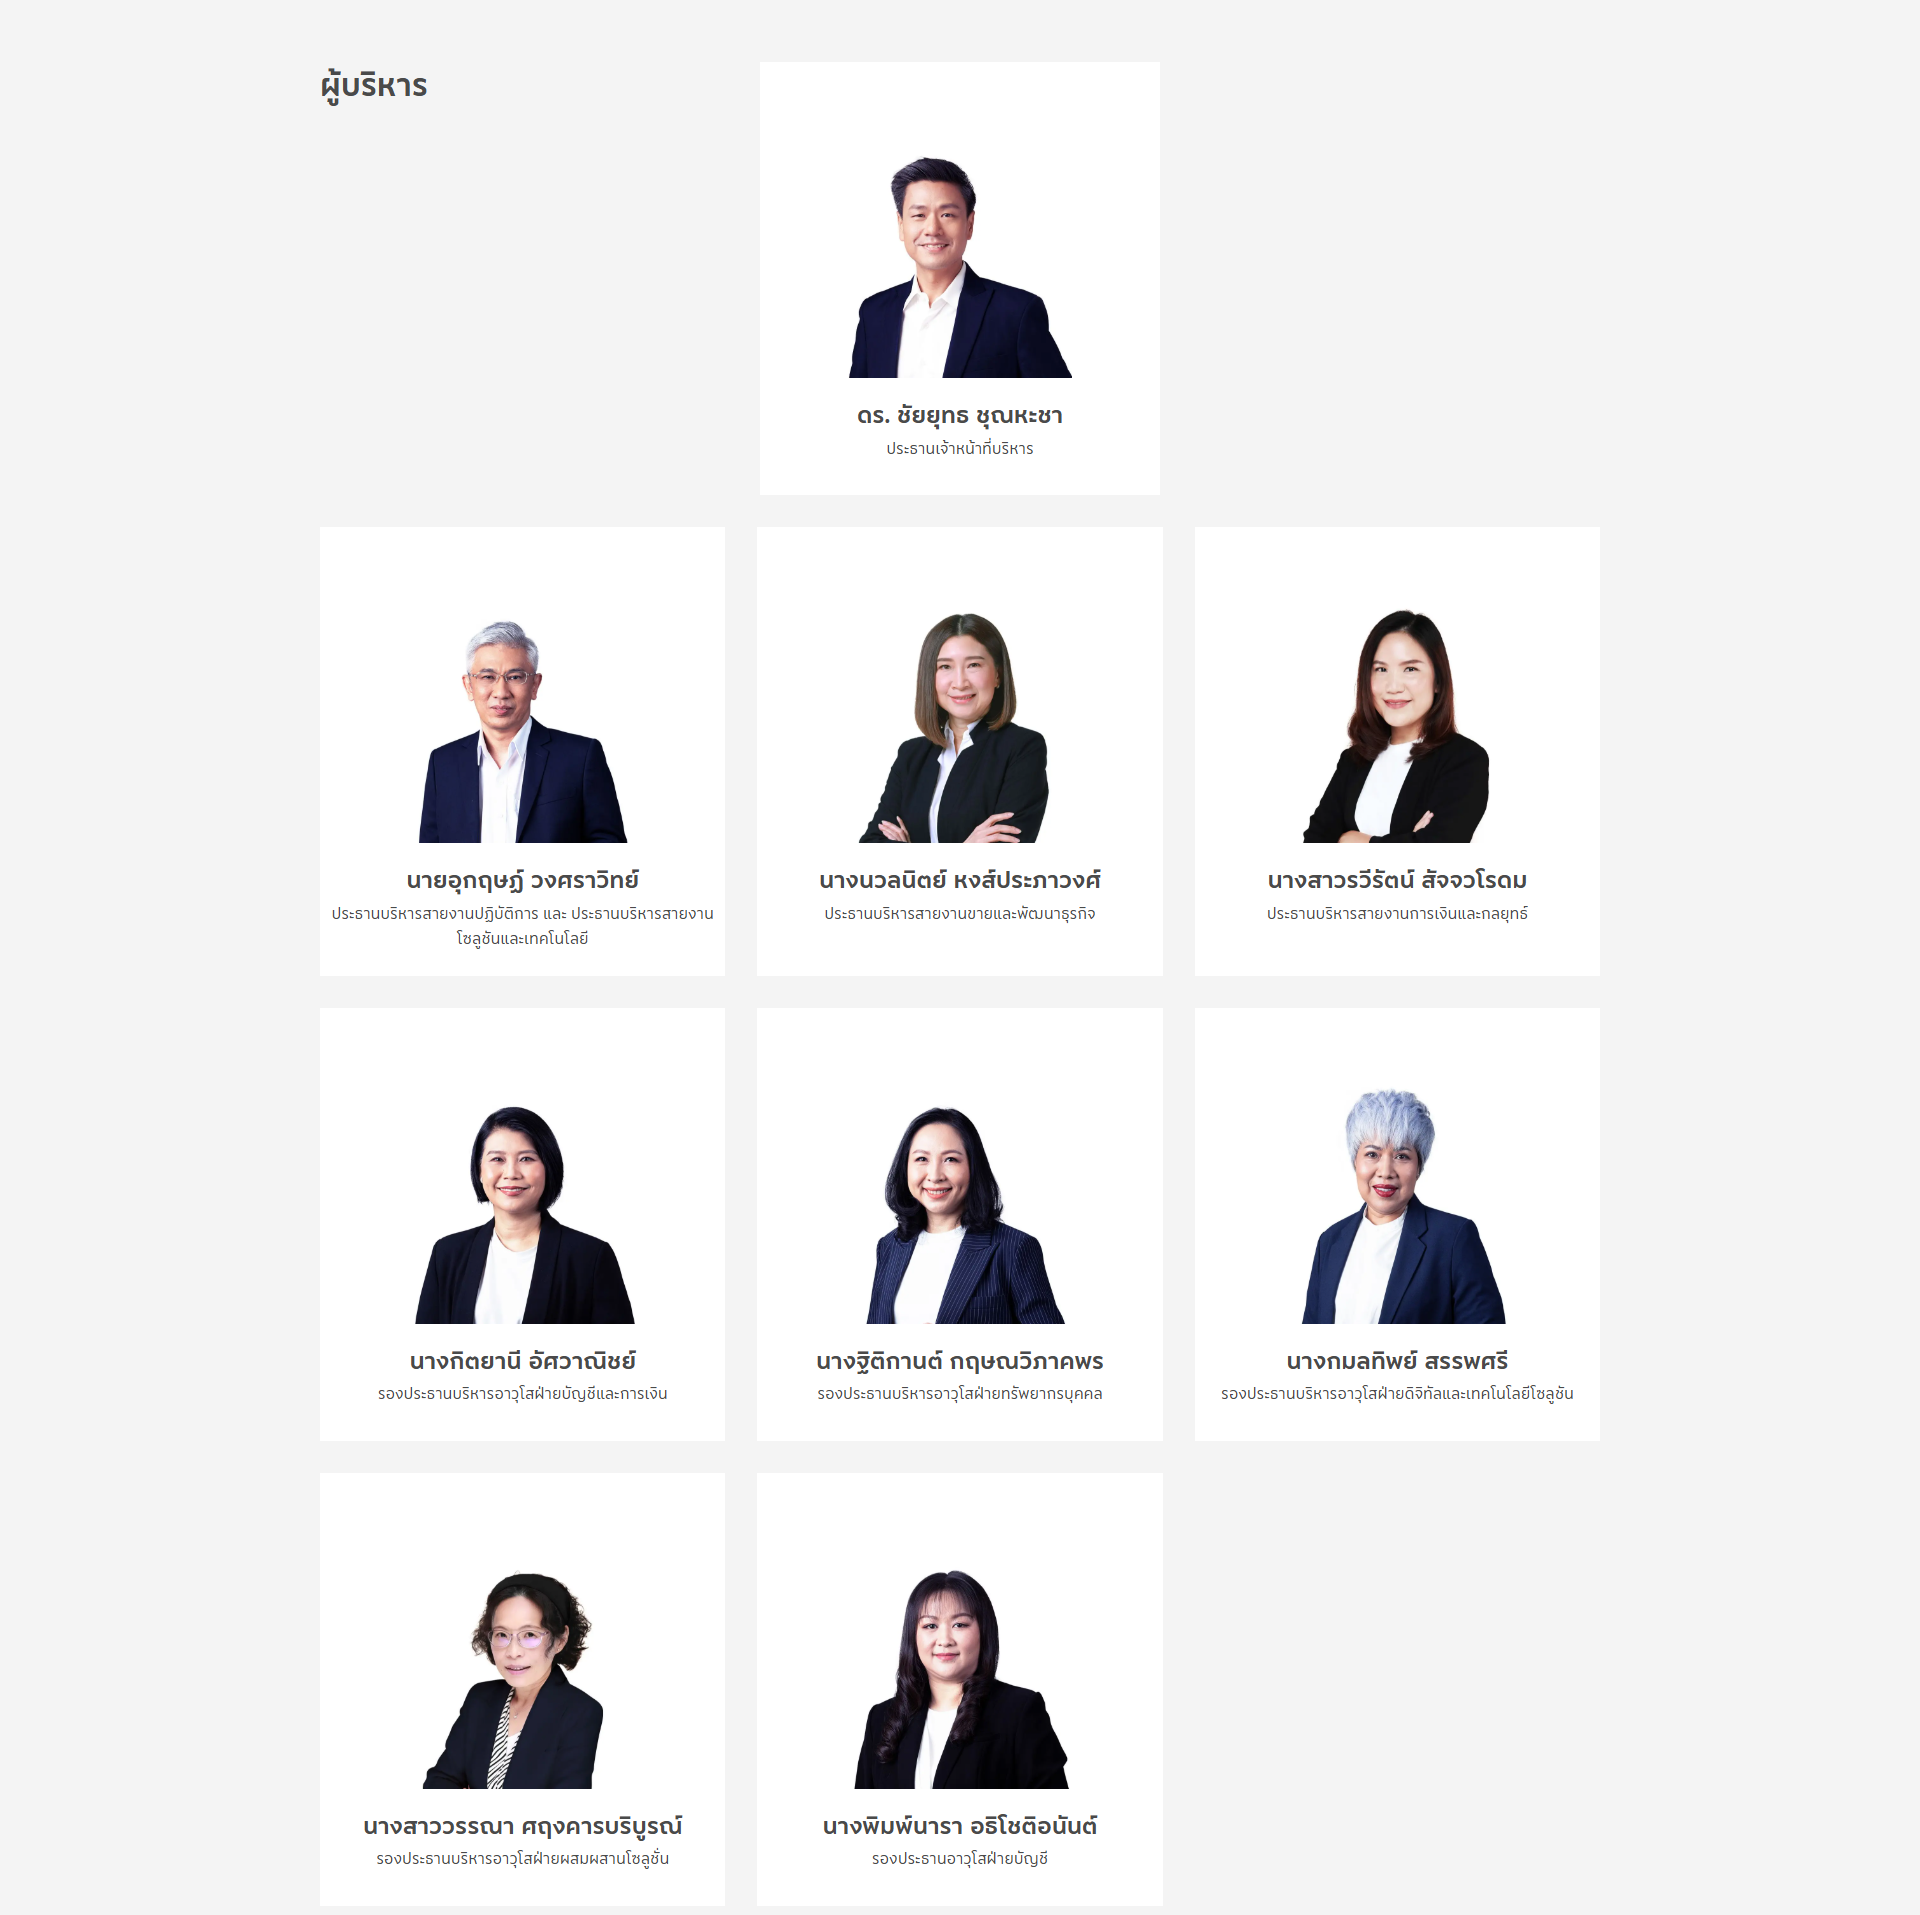
\includegraphics[width=1\linewidth]{./images/g-able-executives.png}
    \end{center}
    \caption[ผู้บริหารและตำแหน่งของบริษัท]{ผู้บริหารและตำแหน่งของบริษัท}
\end{figure}

\clearpage

\section{งบการเงินและงบกำไรขาดทุน}
\subsection{งบการเงิน}
\begin{figure}[ht]
    \begin{center}
        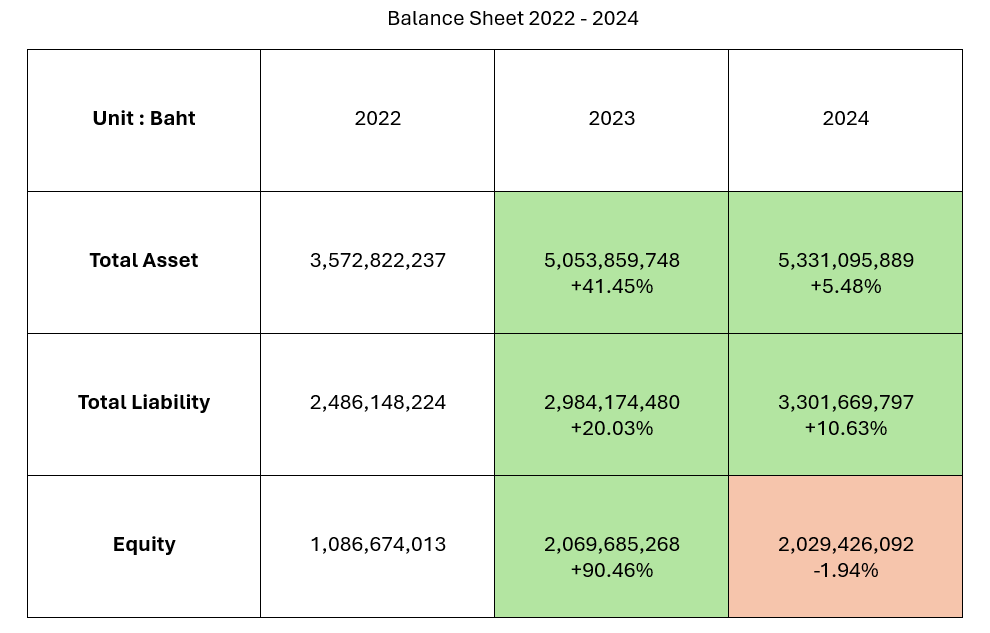
\includegraphics[scale=0.4]{images/balance.png}
    \end{center}
    \caption[งบการเงินย้อนหลังตั้งแต่ก่อตั้งบริษัท]{งบการเงินย้อนหลังตั้งแต่ก่อตั้งบริษัท}
\end{figure}
จากข้อมูลใน \textit{รูปที่ 1.2} จะเห็นได้ว่าบริษัท \textbf{G-Able} มีสินทรัพย์รวมอยู่ที่ 3,573 ล้านบาท ในปี 2022 (ค.ศ. 2022) และเพิ่มขึ้นอย่างรวดเร็วเป็น 5,054 ล้านบาท ในปี 2023 หรือเติบโตประมาณร้อยละ 41.5 ก่อนจะชะลอเป็น 5,331 ล้านบาท ในปี 2024 (+5.5\%) ซึ่งสะท้อนถึงการขยายธุรกิจและการบริหารสินทรัพย์ที่มีประสิทธิภาพ
ในด้านโครงสร้างทุน บริษัทมี \textbf{หนี้สินรวม} เพิ่มจาก 2,486 ล้านบาท เป็น 3,302 ล้านบาท ขณะที่ \textbf{ส่วนผู้ถือหุ้น} เพิ่มจาก 1,087 ล้านบาท เป็น 2,070 ล้านบาท ในปี 2023 ก่อนจะลดเล็กน้อยเหลือ 2,029 ล้านบาท ในปี 2024 แสดงว่าบริษัทสามารถควบคุมหนี้สินได้ดีและยังมีทุนเพียงพอต่อการเติบโต

\textbf{สรุป:} G-Able มีสินทรัพย์สูง โครงสร้างทุนแข็งแรง หนี้สินอยู่ในระดับเหมาะสม และยังคงเติบโตอย่างมั่นคงในระยะยาว

\clearpage


\subsection{งบกำไรขาดทุน}
\begin{figure}[ht]
    \begin{center}
        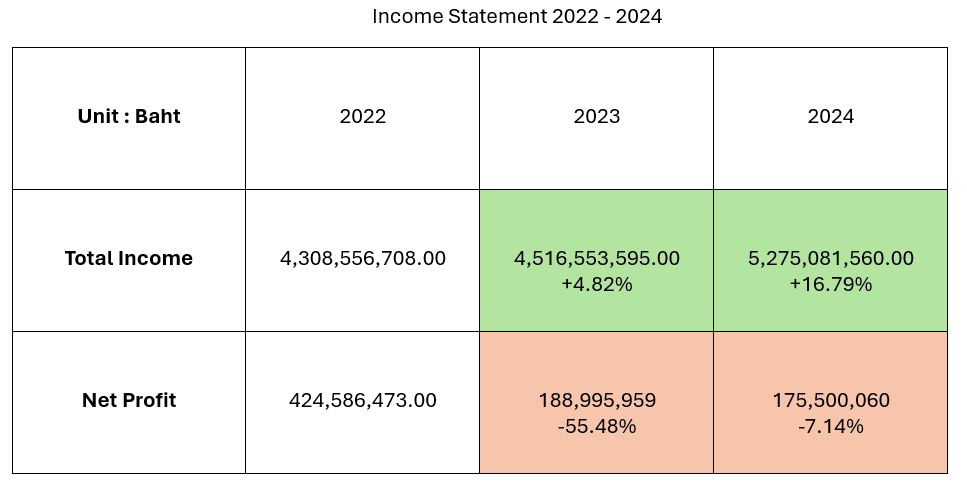
\includegraphics[scale=0.4]{images/income.png}
    \end{center}
    \caption[งบกำไรขาดทุนย้อนหลังตั้งแต่ก่อตั้งบริษัท]{งบกำไรขาดทุนย้อนหลังตั้งแต่ก่อตั้งบริษัท}
\end{figure}

รายได้รวมของบริษัท \textbf{G-Able} ในช่วงปี 2022–2024 เติบโตต่อเนื่องจาก 4,308 ล้านบาท เป็น 5,275 ล้านบาท หรือเฉลี่ยประมาณร้อยละ 10 ต่อปี แสดงถึงการขยายธุรกิจที่แข็งแกร่ง อย่างไรก็ตาม กำไรสุทธิกลับลดลงจาก 425 ล้านบาท ในปี 2022 เหลือ 176 ล้านบาท ในปี 2024 เนื่องจากต้นทุนและค่าใช้จ่ายที่เพิ่มขึ้น

\noindent แนวโน้มในอีก 2–3 ปีข้างหน้า คาดว่ารายได้จะยังเติบโตได้ราวร้อยละ 8–12 ต่อปี โดยอาจแตะระดับ 6,500–7,500 ล้านบาท ขณะที่กำไรสุทธิอาจทรงตัวหรือลดลงเล็กน้อย หากยังไม่สามารถควบคุมต้นทุนได้อย่างมีประสิทธิภาพ ทั้งนี้ การเพิ่มสัดส่วนรายได้จากบริการซอฟต์แวร์และโซลูชันที่มีกำไรสูง จะเป็นกุญแจสำคัญต่อการเติบโตในอนาคต

\clearpage


\section{หน้าที่ของหน่วยงานที่ได้มาสหกิจ}
ในตำแหน่ง Full Stack Developer ที่บริษัท G-ABLE หน้าที่หลักของคือการพัฒนาและปรับปรุงระบบทั้งส่วนหน้า (Front-end) และส่วนหลัง (Back-end) ของเว็บแอปพลิเคชัน โดยมุ่งเน้นให้ระบบทำงานได้อย่างมีประสิทธิภาพและตอบสนองต่อความต้องการของผู้ใช้

นอกจากนี้ ยังได้ทำงานร่วมกับทีม UX/UI เพื่อปรับปรุงประสบการณ์การใช้งานของผู้ใช้ (User Experience) และออกแบบส่วนติดต่อผู้ใช้ (User Interface) ให้ใช้งานได้สะดวกและสวยงาม รวมถึงทำงานร่วมกับทีม QA (Quality Assurance) เพื่อทดสอบ ตรวจสอบ และแก้ไขข้อผิดพลาดของระบบก่อนนำขึ้นใช้งานจริง เพื่อให้มั่นใจว่าระบบมีความถูกต้อง เสถียร และพร้อมใช้งานตามมาตรฐานของบริษัท

% Define groups of JIRA cards
\newcommand{\supportJiraCards}{
  XDO-7387 & CBS-SunCBS | Destroy Dev02 resources \\
  XDO-7389 & CBS-SunCBS Request to add role to managed identity \\
  XDO-7394 & CBS-MCR | Provisioning Storage Account for Dev01 and QA01 \\
  XDO-7421 & CBS-SunCBS | Request to set parameter on MySQL to Off on IaC \\
  *XDO-7422 & CBS-DAP | Setup ADF to send diagnostic log to DAP log analytic workspace \\
  XDO-7429 & Require provision the existing azure manage identity to version v.1.2.1 \\
  *XDO-7444 & CBS-SunCBS Request to install teleport for MySQL flexible servers \\
  XDO-7453 & CBS MCR | Request to grant db\_datareader access to the Azure Automation Account user-managed identity \\
  XDO-7490 & CBS-SunCBS | setup Mysql parameter on QA01 \\
  XDO-7604 & CBS-SunCBS | Provisioning Infrastructure resource for Migration-Dev1 (DEV03) \\
  XDO-7686 & CBS-SunCBS | Asssement of changing Storage account ADLS Gen2 \\
  XDO-7745 & CBS-SunCBS | Change storage account from General to ADLS Gen2 on Dev01 \\
}

\newcommand{\developJiraCards}{
  XDO-7423 & POC ADF Storage Event Trigger Over SFTP
  XDO-7483 & [ADF][linked-services] Convert module from IAC next gen to xplatform multicloud \\
  XDO-7484 & [ADF][trigger] Convert module from IAC next gen to xplatform multicloud \\
  XDO-7561 & CBS-DAP | Enhance Azure Data factory linked services modules \\
  XDO-7633 & [PYMD] Develop check appconfig for Azure Databrick \\
  XDO-7737 & [CBS] Update linked service catalog to support custom sftp \\
  XDO-7742 & [CBS] Create Linked Services documentation \\
  XDO-7743 & CBS-SunCBS | Research on Entra ID with CosmosDB for PostgreSQL \\
  XDO-7744 & [CBS] | POC Dynamic create trigger via ARM Template\\
  XDO-7760 & [CBS] Make the ADF dynamic trigger document \\
  
  XDO-7784 & POC about dataset reference to use in ADF pipeline.
}

% Create a table of JIRA cards with hyperlinks
\newcommand{\jiradata}{
  \begin{center}
    \begin{tabular}{|c|p{0.7\textwidth}|}
      \hline
      \multicolumn{1}{|c|}{\textbf{รหัส Jira Card}} & \multicolumn{1}{c|}{\textbf{หัวข้องาน}} \\
      \hline
      \multicolumn{2}{|c|}{\textbf{Support Cards}}                                         \\
      \hline
      \supportJiraCards
      \hline
      \multicolumn{2}{|c|}{\textbf{Develop Cards}}                                         \\
      \hline
      \developJiraCards
      \hline
    \end{tabular}
  \end{center}
}

% Helper command to create hyperlinks
\newcommand{\jiralink}[1]{\hyperref[desc:#1]{\texttt{#1}}}

\setcounter{secnumdepth}{3}

\chapter{\ifenglish Cooperative Details\else รายละเอียดเกี่ยวกับการทำงาน / ผลการปฏิบัติงาน \fi}

\section{\ifenglish Foundation of Fullstack\else ปรับความรู้พื้นฐานของการเป็น Fullstack\fi}
แนวทางในการเริ่มต้นทำงานในสายงาน Fullstack จำเป็นต้องมีการศึกษาและปรับพื้นฐานความรู้ที่สำคัญเพื่อให้แน่ใจว่าพร้อมสำหรับการทำงานจริง  
เนื่องจาก Fullstack เป็นสายงานที่มีความใหม่และมีการพัฒนาอย่างต่อเนื่องในวงการซอฟต์แวร์ โดยหัวข้อที่ได้รับมอบหมายให้ศึกษาเพื่อเตรียมความพร้อมจะประกอบด้วย

\begin{itemize}
    \item \textbf{Angular}: Framework สำหรับพัฒนา Front-end Web Application แบบ Single Page Application (SPA) ช่วยให้การจัดการ Component, Template, และ Data Binding มีประสิทธิภาพ
    \item \textbf{Java Spring Boot}: Framework สำหรับพัฒนา Back-end Application ช่วยให้สร้าง REST API และจัดการ Business Logic ได้อย่างเป็นระบบ
    \item \textbf{SQL Server}: ระบบฐานข้อมูลเชิงสัมพันธ์ (Relational Database) สำหรับจัดเก็บและจัดการข้อมูลของแอปพลิเคชัน
\end{itemize}

ทั้งนี้การศึกษาหัวข้อเหล่านี้มีระยะเวลาประมาณ 2-4 สัปดาห์ และในท้ายที่สุดจะต้องมีการนำเสนอสิ่งที่ได้เรียนรู้
ให้กับพี่ ๆ ในทีมได้ฟังและประเมิณว่าพร้อมที่จะทำงานจริงหรือไม่ อย่างไรก็ตามรายละเอียดในหัวข้อย่อยต่าง ๆ หลังจากนี้จะเป็นการนำเสนอสิ่งที่ได้เรียนรู้และได้นำมาประยุกต์ใช้ในการทำงานจริง
ส่วนหัวข้อนอกเหนือจากที่จะกล่าวถึงก็สำคัญไม่น้อยเช่นกันแต่จะข้อนำเสนอ Documentation ที่ได้ทำสรุปการเรียนรู้มาแล้วนั้นในส่วนภาคผนวก

\clearpage
\import{chapters/detail_sections}{angular.tex}
\clearpage
\import{chapters/detail_sections}{springboot.tex}
\clearpage
\import{chapters/detail_sections}{sql_server.tex}
\clearpage

\section{\ifenglish TOR\else TOR\fi}

เนื่องจากการมาสหกิจศึกษาจำเป็นต้องมีการประเมินที่เข้มงวด ดังนั้นจึงได้จัดทำ TOR ขึ้นเพื่อเป็นมาตรฐานและข้อตกลงในการทำงาน  
และประเมินผลร่วมกับบริษัทและอาจารย์ เพื่อให้มั่นใจว่างานสามารถทำได้ตามเป้าหมายของ Fullstack Project  

\begin{itemize}
    \item ทำงานในลักษณะของ Task-based โดยกำหนดจำนวนขั้นต่ำของ Task ไว้ที่ 60 tasks  
    เนื่องจากทีม Fullstack ทำงานตามแนวทาง Agile โดยแบ่งงานเป็น Sprint  
    ทุก Sprint จะมีการ Planning เพื่อกำหนดลำดับความสำคัญของ Task  
    และมีการประชุม Weekly-Update ทุกวันพุธเพื่อติดตามความคืบหน้า ทำให้การทำงานมีความรอบคอบและสามารถปรับเปลี่ยนได้ตามความต้องการของ Product Owner และลูกค้า
\end{itemize}
ดังนั้นหัวข้อถัดไปจะเป็นการนำเสนอ Task งานที่ได้รับมอบหมายทั้งหมด เพื่อแสดงให้เห็นว่าสามารถบรรลุเป้าหมายของ TOR ได้ตามแผนงาน Agile

\section{\ifenglish Responsibility Task\else งานที่ได้รับมอบหมาย\fi}

สืบเนื่องจากงานที่ได้รับมอบหมายจะเป็นในลักษณะ Task งาน  
ดังนั้นใน Section นี้จะนำเสนอ Task งานทั้งหมด พร้อมรายละเอียดของแต่ละ Task งาน  
โดยจะแบ่งออกเป็น 3 กลุ่มหลัก ดังนี้:

\begin{itemize}
    \item \textbf{TASK}: งานพัฒนาฟีเจอร์ใหม่หรือทำงานตาม requirement ที่กำหนด
    \item \textbf{CR (Change Request)}: งานปรับปรุงหรือปรับแก้ตามคำขอเพิ่มเติมจากผู้ใช้งานหรือ Product Owner
    \item \textbf{DEFECT}: งานแก้ไขบัคหรือปัญหาที่เกิดขึ้นในระบบ
\end{itemize}
การแบ่งกลุ่ม Task ดังกล่าวช่วยให้สามารถติดตามความคืบหน้าในลักษณะ Agile ได้อย่างชัดเจน  
และสะท้อนถึงความสามารถในการจัดการงานทั้งการพัฒนา การปรับปรุง และการแก้ไขปัญหา

% เรียก Module ทั้งหมด
\subsection{Other Charge Module}

\subsubsection{Task}
\begin{itemize}
    \setlength\itemsep{1em}
    \item \textbf{{GISLOCK-5943 [FA-Other charge request] จัดทำหน้าจอ Other charge request}} \\
          เป็นการเพิ่มโปรแกรมใหม่ในแผนกของการเงิน โดยการเป็นสร้างโปรแกรมที่ชื่อว่า Other Charge Request และ Other Charge Request List\\
          Other Change Request : เป็นโปรแกรมเกี่ยวกับการเรียกค่าใช้จ่ายเพิ่มเติมนอกเหนือจากเบี้ยประกัน \\
          Other Change Request List : เป็นหน้าที่เอาไว้รายการที่เราสร้างไว้
    \item \textbf{{GISLOCK-6755 [Set up Transaction Code] เพิ่มหน้าจอ Set up Transaction Code}} \\
          เป็นการเพิ่มโปรแกรมใหม่ที่เราจะเแาไว้ตั้งค่ารายการ Transaction Code ที่จะใช้ในโปรแกรม Other Charge Request กับ Other Expense Request \\
          โดยจะแบ่ง 2 โปรแกรมคือ Set up Transaction Code และ Set up Transaction Code List 
    \item \textbf{{GISLOCK-7019 [Other Charge] เพิ่มปุ่ม Update (สำหรับ Refresh) ข้อมูล Installment และ ShareDept}} \\
          เป็นการเพิ่มปุ่ม Update ในหน้าจอ Other Charge Request เพื่อให้ผู้ใช้สามารถกดปุ่มนี้เพื่อรีเฟรชข้อมูลในตาราง Installment และ Share Department ได้ แบบอัตโนมัติ
    \item \textbf{{GISLOCK-7106 [Other Charge] แก้ไขโปรแกรม Other charge Request List เพิ่มเงื่อนไขในการ query เพื่อค้นหาข้อมูลโดยกรองเฉพาะ Entry\_by ที่ตรงกับ User Login}} \\
          เป็นการแก้ไขโปรแกรม Other Charge Request List โดยเพิ่มเงื่อนไขในการค้นหาข้อมูลให้สามารถกรองเฉพาะ Entry\_by ที่ตรงกับ User Login นั้น ๆ ได้ \\
          อนาคตจะแบ่งให้แสดงแค่แผนกที่ตัวเองรับผิดชอบ
    \item \textbf{{GISLOCK-7200 [Other Charge] แก้ไขโปรแกรม Charge Request ส่วนของการ Share dept \, Installment}} \\
          ปรับการแสดงข้อความเตือน เมื่อมีการกรอกข้อมูลไม่ครบถ้วนในส่วนของ Share Department และ Installment \\
          โดยจะมีการเช็คให้ข้อมูลของ Installment และ Share Department ต้องมีค่าเปอร์เซ็นต์รวมกันเท่ากับ 100\% ถึงจะสามารถบันทึกข้อมูลได้ \\
          และจะต้องมีจำนวนเงินที่สัมพันต์กับจำนวนเงินใน Transaction ด้วย
    \item \textbf{{GISLOCK-7289 [Other Charge] Set up Transaction Code เพิ่ม DropdownFlag}} \\
          เป็นการเพิ่มตัวเลือก DropdownFlag ในหน้าจอ Set up Transaction Code \\
          เพื่อให้ผู้ใช้สามารถเลือกได้ว่ารายการ Transaction Code ที่สร้างขึ้นมานั้น จะนำไปแสดงในหน้าจอ Other Charge Request หรือไม่
    \item \textbf{{GISLOCK-7688 [Other Charge] Other Charge Request Booking}} \\
          เป็นการเพิ่มโปรแกรมในส่วนของแผนกการเงิน เป็นโปรแกรมที่แผนกการเงินจะเอาไว้ตรวจสอบหรือแก้ไขรายการที่ถูกอนุมัติแล้ว \\
          โดยจะมีการแยกเป็น 2 โปรแกรมคือ Other Charge Booking และ Other Charge Booking List
    \item \textbf{{GISLOCK-7689 [Other Charge] Other Charge Request บันทึกขาคู่}} \\
          เป็นส่วนหนึ่งของโปรแกรม Other Charge Request ที่เพิ่มขึ้นมา \\
          โดยจะเป็นการบันทึกข้อมูลแบบขาคู่ คือการที่เราจะต้องบันทึกข้อมูลทั้งในฝั่งของ Other Charge Request และ Other Expense Request พร้อมกัน \\
          โดยจะมี 2 แบบ คือ : \\
            1. แบบ auto ที่จะสร้าง Other Expense Request ให้อัตโนมัติเมื่อมีการบันทึก Other Charge Request \\
            2. แบบ manual ที่จะให้ผู้ใช้เป็นคนเลือกว่าจะสร้าง Other Expense Request ด้วยตัวเอง
\end{itemize}

\subsubsection{Defect}
\begin{itemize}
    \setlength\itemsep{1em}
    \item \textbf{{GISLOCK-5457 [Other Charge] ปรับการแสดงผลข้อมูลในส่วน Bill to ให้ไปในทางเดียวกับ AP}} \\
          เพิ่มการ Clear โดยการกดปุ่ม X ที่ Bill To
    \item \textbf{{GISLOCK-6189 [Other Chare/Expense] Standard Search Search like เวลาเก็บ Data ใน DB ให้คั่นด้วย Space Bar}} \\
          1.ปรับตรง placeholder ของการ Search เราจะเอาการเว้นวรรคออก จะแสดงชิดกันเลย โดยมี / คั่น
          2.ตรง Database จะปรับจากการเก็บที่คั่นโดย | มาใช้เป็น " " (Spacebar หรือ การเคาะช่องว่างแทน) 
    \item \textbf{{GISLOCK-6518 [FA- Other charge request] ปรับ feature ทำหน้าจอ Other charge request}} \\
          เป็นการแก้หลายๆ จุดในโปรแกรม Other Charge Request ที่ได้มีการพัฒนาขึ้นมา \\
            โดยมีการปรับปรุงดังนี้ \\
            1. ปรับปรุงการแสดง ปุ่ม Add/Clear ของส่วน Share Department ให้ตำแหน่งปรับตำขนาดหน้าจอ\\
            2. ปรับปรุงหน้า Approve เมื่อกด view mode มาต้องไม่มีปุ่ม Add/Clear ของแต่ละส่วนแสดง \\
            3. view mode ที่กดมาจากหน้า List ส่วนของ Transaction จะต้องเอาข้อมูลของชุดแรกมาแสดง \\
            4. Hq/Branch แสดงเป็นข้อมูล ไม่ต้องแสดงโค้ด \\
            5. Exchange Rate ใน Transaction ให้แสดง 8 ตำแหน่ง \\
            6. เมื่อเราเพิ่ม Transaction แล้วเราจะทำการปิด Currency/Exchange Rate ไม่ให้แก้ไขได้ เพื่อ Transaction ต่อไปจะได้ Currency/Exchange Rate เหมือนกัน\\
            7. กรณีที่เรามี Installment หรือ Share Department แล้วเราไปแก้ไข Transaction เมื่อจะเซฟเราจะต้องเตือนบอกว่า Transaction มันเปลี่ยนแปลง และเซฟไม่ได้ 
    \item \textbf{{GISLOCK-6561 [Other Charge] Pop up \: Bill To แสดงข้อมูลเดียวกัน ซ้ำๆ}} \\
          สาเหตุที่ข้อมูลแสดงซ้ำ เนื่องจากมีการเชื่อมโยง (JOIN) กับตารางข้อมูลอื่น เช่น ตารางที่อยู่ (Address) ซึ่งมีหลายรายการต่อรหัสลูกค้าหรือพาร์ทเนอร์ ทำให้ข้อมูลหลักหนึ่งรายการถูกแสดงซ้ำตามจำนวนข้อมูลที่อยู่ที่สัมพันธ์กันในตารางดังกล่าว \\
          วิธีแก้ไขคือ การปรับคำสั่ง SQL ที่ใช้ในการดึงข้อมูล โดยการใช้คำสั่ง DISTINCT เพื่อให้แสดงเฉพาะรายการที่ไม่ซ้ำกัน หรือการปรับโครงสร้างการ JOIN ให้เหมาะสมกับความต้องการของข้อมูลที่จะแสดง
    \item \textbf{{GISLOCK-6563 [Other Charge] Contact Information จะต้องดึงข้อมูลมาจาก Contact Person ของ Client หรือ Partner มาแสดงโดย link up กับ Bill to ที่ได้เลือก}} \\
          ปรับปรุงตรง Contact Information :\\
          1.ดึงข้อมูลมาแสดงอัตโนมัติตาม Main Contact \\
          2.กรณีมีหลาย Contact เปลี่ยนได้กดเปลี่ยนตรง modal จะมี Contact ที่สามารถเปลี่ยนได้
    \item \textbf{{GISLOCK-6566 [Other Charge] ปรับ wording ของชื่อฟิลด์ ทั้งหน้า Request และ List}} \\
          เป็นการแก้ไขคำของหน้า Request และ List
    \item \textbf{{GISLOCK-6568 [Other Charge] ตรวจสอบการ Save Draft ใบงานและการแสดงค่าเริ่มต้นฟิลด์ Status}} \\
          เพิ่มการเช็คตอนจะ Save Draft ใบคำขอ ให้เช็คว่าเราเลือกตัวที่ต้อง require หรือยัง ถ้ายังให้แจ้งเตือน \\
          และปรับการแสดงค่าเริ่มต้นของฟิลด์ Status ให้แสดงเป็น "Save Draft" เมื่อสร้างใบคำขอใหม่
    \item \textbf{{GISLOCK-6571 [Other Charge] ส่วน Share Department ปรับการแสดงปุ่ม Add \, Clear และเมื่อเลือกข้อมูล Department รูปแบบฟอร์มต้องไม่ขยับไปมา}} \\
          ปรับปรุงการแสดงปุ่ม Add และ Clear ในส่วนของ Share Department ให้มีตำแหน่งที่คงที่ ไม่ขยับไปมาเมื่อมีการเลือกข้อมูล 
    \item \textbf{{GISLOCK-6575 [Other Charge] การใช้งานปุ่ม View ในส่วน Other Charge Transaction}} \\
          เพิ่มปุ่ม Back ในหน้าจอ View ของส่วน Other Charge Transaction \\
          เพื่อให้ผู้ใช้สามารถกลับไปยังหน้าจอก่อนหน้าได้อย่างสะดวก
    \item \textbf{{GISLOCK-6576 [Other Charge] กรณี Total Amount ใน Transaction และ Installment มียอดไม่เท่ากัน เมื่อ Save \, Submit จะต้องมี Pop up ถาม}} \\
          เมื่อ Total Amount ในส่วนของ Transaction และ Installment มียอดไม่เท่ากัน \\
          ระบบจะต้องแสดง Pop-up แจ้งเตือนผู้ใช้ว่า ยอดรวมไม่ตรงกัน และให้ผู้ใช้ทำการตรวจสอบและแก้ไขข้อมูลก่อนที่จะทำการ Save หรือ Submit ใบคำขอ
    \item \textbf{{GISLOCK-6577 [Other Charge List] ปรับการใช้งาน Request Date From / To}} \\
          1.เพิ่มตรง Coondition Search โดยการเพิ่มการค้นหาด้วย Status 
          2.ไม่ Default วันที่ให้ตอนเริ่มเพราะให้มาเลือกเอง
    \item \textbf{{GISLOCK-6578 [Other Charge List] ฟิลด์ Bill To กดแล้วไม่แสดง Pop up และขอความหมายของ Request No. Running No. C2568XXXXX}} \\
          สาเหตุที่กดแล้วไม่แสดง Pop-up เกิดจากการที่เราไปเรียก id ของ Pop-up นั้นไม่ถูกต้อง
    \item \textbf{{GISLOCK-6583 [Other Charge List] ไม่แสดงข้อมูล Bill to Name}} \\
          เกิดจากการที่ก่อนหน้านี้มีการเก็บข้อมูล Bill to Name ในตารางที่ไม่ถูกต้อง \\
          วิธีแก้ไขคือ ตอนที่เราจะเซฟใบงานเราจะเลือกให้ถูกฟิลด์พอตอนจะเรียกมาหน้า List ก็จะได้ข้อมูลที่ถูกต้อง
    \item \textbf{{GISLOCK-6589 [Other Charge List] การใช้งานและความหมายของ Submit Date}} \\
          เพิ่มคำอธิบายใต้ฟิลด์ Submit Date ในหน้า Other Charge List 
    \item \textbf{{GISLOCK-6591 [Other Charge] ปรับชื่อฟิลด์ Entry By และ Entry Date ให้กับหน้าจอ Request และ List}} \\
          เปลี่ยนมาใช้ชื่อฟิลด์เป็น Entry By และ Entry Date ในหน้าจอ Request และ List 
    \item \textbf{{GISLOCK-6592 [Other Charge List] เพิ่มการแสกงข้อมูลในคอลัมน์ Invoice Date}} \\
          เพิ่มการแสดงข้อมูลในคอลัมน์ Invoice Date ในหน้า Other Charge List 
    \item \textbf{{GISLOCK-6649 [Other Charge][Request Other Charge] ปรับการทำงานส่วน Contact Information ให้มีฟังก์ชันการทำงานเหมือนกับ AP}} \\
          ปรับการทำงานตามนี้ \: \\
          1. เมื่อเลือก Bill to Code แล้วให้ดึงข้อมูล Contact Information มาแสดงอัตโนมัติ โดยเลือกจาก All Purpose เป็นลำดับแรก \\
          2. หากมีหลาย contact สามารถกดปุ่มแว่นขยายเพื่อแสดง modal ของ contact ที่มีหลายอันแล้งเลือกได้
    \item \textbf{{GISLOCK-6675 [Other Charge][Request Other Charge] ส่วน Request Information ทำการ Edit ข้อมูลในตารางแต่ระบบไม่ Update ตาม}} \\
        เกิดจากการที่เราส่งข้อมูลไปแต่ว่าไอดีในการอัปเดตข้อมูลนั้นไม่ถูกส่งไป เลยไม่รู้ว่าจะแก้ไขที่ข้อมูลไหน ทำการแก้ไขโดยการส่งไอดีเพิ่มไปด้วย
    \item \textbf{{GISLOCK-6773 [Other Charge][Request Other Charge] Submit ใบงาน ระบบแสดง The sum of all tables is not equal.}} \\
        เพิ่มการแสดง Modal เมื่อผลรวมของ Total Amount ไม่เท่ากันใน Installment และ Share Department
    \item \textbf{{GISLOCK-6877 [OTC][Request Other Charge] กรณีเลือก Edit รายการเพื่อตรวจสอบข้อมูล แต่ Entry Date แสดงเป็นวันที่ปัจจุบัน ซึ่งไม่ถูกต้องให้แก้ไขเป็นวันที่บันทึกใบงานตั้งต้น}} \\
        จากเดิมก่อนหน้านี้เป็นการ mock up ข้อมูลมาเลยทำให้การแสดงเป็นวันปุจจุบันเสมอ เราจะแก้ไขใน mode edit ให้ไปดึงข้อมูลจากฐานข้อมูลมาแสดงแทน
    \item \textbf{{GISLOCK-6878 [OTC][Request Other Charge] กรณีเลือก Invoice Name ฟิลด์ Invoice Address จะต้องแสดงข้อมูลที่สัมพันธ์กับ Name ที่เลือก}} \\
        ปรับปรุงการทำงานของฟิลด์ Invoice Address ให้แสดงข้อมูลที่สัมพันธ์กับ Invoice Name ที่ผู้ใช้เลือก \\
        โดยการเชื่อมโยงข้อมูลจากฐานข้อมูลเพื่อดึงที่อยู่ที่ตรงกับชื่อที่เลือกมาแสดง
    \item \textbf{{GISLOCK-6945 [Other Charge List] ปรับการแสดง Location และ Nationality กรณี Bill To เป็นข้อมูลเก่า โดยระบบต้องแสดงข้อมูลที่ได้เลือกจากตอนบันทึก}} \\
        เดิมทีเรามีการเก็บ เป็นคำ location ประมาณนี้แต่เรามีการปรับรูปแบบใหม่ให้เป็นเป็นคีย์ L แบบนี้แทน เราเลยมีเขียน sql เพื่อดึงข้อมูลเดิมมาแล้วดักเคสที่ส่งออกไป ตอนเราจะดึงข้อมูลมาแสดงก็จะได้ข้อมูลใหม่ที่เป้น คีย์ L แทน\\
        แล้วตอนเซฟเราก็จะเซฟเป็นคีย์ L ไปเลย ทำให้เป็นการอัปเดตข้อมูลให้เป็นรูปแบบใหม่ทั้งหมด
    \item \textbf{{GISLOCK-6953 [Other Charge] 1.แก้ไขการแสดง Request Information 2.แก้ไขการแสดง Currency/Exchange Rate 3.แก้ไขการแสดง Bill to Code}} \\
        1. เมื่อทำการกด Icon Edit ข้อมูล Transaction Code ในตารางและไปกดปุ่ม Request Information ข้อมูลเดิมจะต้องไม่หาย \\
        2. เมื่อ Edit เข้ามาจากหน้า List ถ้ามี Transaction อยู่เราจะ Disable Currency และ Exchange Rate เพราะจะใช้ตามอันที่มี
        3. เมื่อ x กากบาท Code หรือ x กากบาท Pop up จะต้องเรียก Service ใหม่ทุกครั้ง เป็นการ refresh ทุกครั้งที่เรากดมาใหม่
    \item \textbf{{GISLOCK-7031 [Other Charge] ปรับการทำงานปุ่ม Submit และ Save Draft}} \\
        จากเดิมเมื่อเป็น view mode ปุ่ม Submit กับ Save Draft มันจะ Disable แต่ยังกดและทำงานได้ \\
        เราเลยปรับให้ปุ่มมันกดไม่ได้เลยเมื่อเป็น view mode 
    \item \textbf{{GISLOCK-7064 [Other Charge] เมื่อ Submit and Save Draft ข้อมูลที่บันทึกไว้ในหน้าจอต้องไม่เคลียร์และ Redirect to List}} \\
        จากอันเดิมก่อนหน้านี้พอเรากด Submit หรือ Save Draft ข้อมูลมันจะเคลียร์ออกจากหน้าจอและนำทางไปสู่หน้าลิสต์ \\
        เราเลยปรับให้เมื่อกด Submit หรือ Save Draft ข้อมูลที่บันทึกไว้ยังคงอยู่ในหน้าจอ และจะ Redirect to List เฉพาะเมื่อผู้ใช้เลือกที่จะกลับไปยังหน้าลิสต์ด้วยตัวเอง
    \item \textbf{{GISLOCK-7144 [Other Charge List] ยอด Amount แสดงไม่ตรงกับการบันทึกในหน้า Request}} \\
        เปลี่ยนจากเดิมเราจะใช้ผลรวมของ Amount ในตาราง Transaction มาแสดง \\
        เป็นการไปดึงยอดผลรวมของ Total Amount มาแสดงแทน
    \item \textbf{{GISLOCK-7215 [Other Charge] ตรวจสอบการคำนวณ Payment Due Date ให้ตรงตามเงื่อนไข}} \\
        ปรับปรุงการคำนวณ Payment Due Date ในหน้าจอ Other Charge Request \\
        โดยจะมีเงื่อนไขดังนี้ \\
        1. การคิด Payment Due Date จะเป็น วันที่สร้างใบคำขอ + payment term ของคนนั้นๆ แต่ถ้าไม่มีจะเป็นค่าเริ่มต้นให้ 30 วัน\\
        2. ถ้า Payment Due Date ตรงกับเสาร์อาทิตย์ และ วันหยุดนักขัตฤกษ์ จะเลื่อนไปเป็นวันทำการถัดไปโดยอัตโนมัติ
    \item \textbf{{GISLOCK-7219 [Other Charge] เพิ่มการแจ้งเตือน Share Department และ Installment กรณีที่ Share (\%) มีจำนวน 0.00 และมากกว่า 100.00}} \\
        ปรับการแจ้งเตือนจากเดิมไม่มีจุดทศนิยม \\
        เป็นการเพิ่มจุดทศนิยม 2 ตำแหน่งในการแจ้งเตือนเมื่อ Share (\%) มีจำนวน 0.00 และมากกว่า 100.00 \\
        เพิ่มการดักเคสที่กรอกค่าเกิน 100.00 และน้อยกว่า 0.00 หรือเท่ากับ 0.00
    \item \textbf{{GISLOCK-7230 [Other Charge] แก้ไขการกดปุ่ม Clear และ เพิ่ม Popup has been saved ให้กับการเพิ่มข้อมูลลงตาราง}} \\
        เพิ่มการแสดง modal เมื่อ add update และ delete เพื่อบอกว่าทำเสร็จแล้วของ Transaction , Request Information , Share Department , Installment
    \item \textbf{{GISLOCK-7241 [Other Charge] ลบรายการ Transaction ออกไปแล้ว ข้อมูลส่วน Installment และ ปุ่ม Update ยังแสดงอยู่ในหน้าจอ}} \\
        เพิ่มการเช็คตอนที่เราจะเซ็ตค่าใหม่ให้อัปเดตตามเงื่อนไข
    \item \textbf{{GISLOCK-7243 [Other Charge] กดปุ่ม Update แล้วไม่ Update ข้อมูล กรณี Installment และ Share Dept มีข้อมูลทั้งคู่}} \\
        เกิดจากการที่เราส่ง payload ไปให้หลังบ้านไม่ถูกเลยทำให้การอัปเดตทำงานไม่ถูกต้อง \\
        แก้ไขโดยการปรับ payload ก็จะสามารถอัปเดตได้ปกติ
    \item \textbf{{GISLOCK-7258 [Other Charge] เพิ่มการปรับ \% ของ Share Department และ Installment}} \\
        เพิ่มการคำนวณเปอร์เซ็นต์ให้อัตโนมัติเช่น เริ่มต้นเรามี 100 แล้วเราเพิ่มอันแรกไป 20 แล้วมันก็จะเหลือ 80 ให้ใช้ครั้งต่อไป รวมถึงการคำนวณ total amount ด้วย
    \item \textbf{{GISLOCK-7395 [Other Charge] เมื่อเลือก Vat Calculation = Non Vat ให้ Disable Field 1.Vat Type 2.Vat Rate \% 3.Vat Amount}} \\
        จะทำการปิดฟิลด์ดังกล่าวเมื่อเลือก Vat Calculation เป็น Non Vat
    \item \textbf{{GISLOCK-7419 [Other Charge] ส่วน Contact Information เพิ่มเงื่อนไขเมื่อไม่มีการเลือก Code ให้ Disable ส่วน Contact ไว้ก่อนเสมอ}} \\
        ปรับปรุงให้เมื่อเราเข้ามาครั้งแรกตอนที่เรายังไม่เลือก ลูกค้าหรือพาร์ทเนอร์ เราจะ Disable ส่วนของ Contact ไว้ก่อน
    \item \textbf{{GISLOCK-7439 [Other Charge] Vat Rate \% = 0 ให้ Disable Vat Amount}} \\
        ใน Transaction เราเราเลือก Vat Rate เป็น 0 gik0tmedki Disable Vat Amount ไปเลย เพื่อจะได้ไม่สามารถแก้ไขได้เพราะเราเลือก 0 แล้ว 
    \item \textbf{{GISLOCK-7487 [Other Charge] ตรวจสอบการค้นหาข้อมูลแบบ ค้นหามีช่องว่างระหว่างคำ}} \\
        ปรับรูปแบบการ search ใหม่ จากเดิมเราจะ search ได้ทีละตัว แต่เราจะทำการเพิ่มไป เป็นการ search แบบหลายตัว เช่น "AA BA" \\
        เราจะแสดงผลลัพธ์ที่ตรงกับ AA มาทั้งหมดก่อน ต่ามด้วย BA ต่อด้วย
    \item \textbf{{GISLOCK-7494 [Other Charge] ปรับตำแหน่งการแสดงปุ่ม Search และ Clear}} \\
        ปรับตำแหน่งการแสดงปุ่ม
    \item \textbf{{GISLOCK-7498 [Other Charge] Set up Transaction Code แก้ไขตามรายการ}} \\
        1. Account Code ทำเป็น * ฟิลด์เพื่อป้องปันการ Add ลงตารางโดยที่ไม่เลือกข้อมูล \\
        2. เพิ่มการทำงานของปุ่ม Clear หลัก \\
        3. ปรับ Icon : edit, delete ให้ตรงกับโปรแกรม Standard \\
        4. Account Code จะต้องแสดงแด่ Code และ Account Name สามารถดูได้อย่างเดียวไม่สามารถแก้ไขได้ \\
        7. ปรับฟิลด์ Type มาเป็น Transaction Type ตามหน้า List
        8. เพิ่มการ Validate WHT Rate * และเป็น require field
    \item \textbf{{GISLOCK-7529 [Other Charge] โปรแกรม Set up Transaction Code ทำการ Delete รายการในตารางแล้ว รายการไม่ถูกลบไป}} \\
        ปัญหาเกิดจาก Race Condition คือคำสั่ง GET ทำงานก่อนที่คำสั่ง DELETE จะเสร็จสมบูรณ์ ทำให้เห็นข้อมูลที่ยังไม่ถูกลบจริง \\
        รอให้การลบเสร็จสิ้นก่อนดึงข้อมูล หรือใช้ Transaction/Locking เพื่อควบคุมลำดับการทำงานไม่ให้คำสั่งชนกัน.
    \item \textbf{{GISLOCK-7554 [Other Charge] ลบรายการที่มี Vat Amount ที่ส่วน Transaction ออกไปแล้ว แต่ในส่วน Installment ยังค้างยอด Vat Amount เก่าไว้}} \\
        เกิดจากการที่เราทำการแก้ไขใน Transaction แล้วในส่วนของ Installment ไม่ได้รู้ว่ามันเปลี่ยน เลยแก้ไขโดยการสร้างฟังก์ชันที่จะเช็คว่าถ้ามีการเปลี่ยนแปลงและเข้าเงื่อนไขที่เราตั้งก็จะไปทำฟังก์ชันนี้ก็จะสามารถทำงานได้ปกติ
    \item \textbf{{GISLOCK-7587 [Other Charge] Set up Transaction Code เปลี่ยนจากปุ่ม Submit/Clear เป็น Save/Clear}} \\
        เปลี่ยนหน้า Ui ของปุ่ม
    \item \textbf{{GISLOCK-7626 [Other Charge] เปลี่ยนจากการส่งข้อมูลแบบ queryParams เป็นแบบ getState}} \\
        ปรับจากเดิมที่เป็นการรับมาจาก Params เราปรับเปลี่ยนมาใช้ในรูปแบบ State ซึ่งปลอดภัยและใช้งานได้ดีกว่า
    \item \textbf{{GISLOCK-7628 [Other Charge] ปรับ status เป็นตัวกลางเพื่อให้ sort จะได้ เนื่องจากตอนนี้เป็นการใช้เงื่อนไขในการแปลงจาก code เป็น word และนำมาแสดง ไม่ใช่การ Join}} \\
        เพิ่ม status ของ Other Charge ให้ไปเป็น Workflow ของตัวกลางเพื่อที่จะได้เข้ากระบวนการ approval ของส่วนกลาง และ จะสามารถนำมา Sort ได้
    \item \textbf{{GISLOCK-7629 [Other Charge] ลบข้อมูลในตาราง Installment แล้วในตาราง Transaction มีแต่เคส VATNO ระบบไม่ Disable Field Vat ในส่วน Installment ให้}} \\
        เกิดจากตอนที่เรา แก้ไขข้อมูลใน Installment แล้วเราไม่ได้เช็คของ Transaction เลยทำให้ตอนเราลบแล้วจะเซ็ตใหม่เลยกลับมาเปิด Vat Amount ทั้งๆที่ใน Transaction ยังมี VATNO \\
        เราแก้ไขโดยการเพิ่มการเช็คไปตอนเราเคลียร์เพื่อจะเซ็ตใหม่ ก็จะทำให้ฟิลด์เปิดปิดตามข้อมูล Transaction ที่เรามี
    \item \textbf{{GISLOCK-7631 [Other Charge][Set up Transaction Code] Mode Edit ข้อมูลที่เคยบันทึกไว้ เช่น WHT Rate กับ Show Trans code ไม่ตรงกับที่บันทึก}} \\
        ปัญหานี้เกิดจาก type ของ ฟิลด์ WHT Rate ไม่ตรงกับ Database \\
        เราเลยแก้ไขโดยการปรับ type ของฟิลด์ WHT Rate ให้ตรงกับ Database ก็จะสามารถดึงข้อมูลมาแสดงในโหมด Edit ได้ถูกต้อง
    \item \textbf{{GISLOCK-7694 [Other Charge] แก้ไขการค้นหาช่วงวันที่ Date From และ Date To ให้ตรงกับช่วงที่ค้นหา}} \\
        จากเดิมตอนเราเลือกใน format เป็น ISO 8601 อาจมีปัจจัยเรื่อง Timezone เข้ามาเกี่ยวข้องทำให้การค้นหาไม่ตรงกับช่วงวันที่ที่เลือก \\
        เราเลยแก้ไขโดยปรับเป็นรูปแบบ dd/mm/yyyy แทน ทีนี้ก็จะไม่มีปัญหาเรื่อง Timezone แล้ว ก็จะทำให้การค้นหาตรงกับช่วงวันที่ที่เลือก
    \item \textbf{{GISLOCK-7737 [Other Charge] Set up Transaction Code List กดปุ่ม Add แล้วไม่แสดงหน้าจอ Set up Transaction Code}} \\
        เรามีการปรับจากเดิมที่มีการใช้ getParam มาเป็นการใช้ getState \\
        พอเรากด Add มาจากหน้า List อาจทำให้ State ที่ส่งมาไม่ครบ เราเลยแก้ไขให้ตอนกด Add มันจะไม่เอา State อะไรมาส่งเลย ทำให้มัน Redirect มาที่หน้า Set up Transaction Code List ปกติ \\
        แก้ไขโดยการ set ค่า default ให้กับ State ที่ขาดหายไป 
    \item \textbf{{GISLOCK-7793 [Other Charge] ส่วน Share Department ขาดการแสดงคอลัมน์ Department Name ที่ตารางแสดงผล}} \\
        เพิ่มส่วนของ Department Name ในตารางแสดงผลของ Share Department \\
        โดยการดึงข้อมูลชื่อแผนกจากฐานข้อมูลมาแสดงในตาราง
    \item \textbf{{GISLOCK-7807 [Other Charge] OTC List กด link condition search และกดปุ่ม search ระบบแจ้งเตือน Invalid column name 'OTC\_BILLTO\_CD'.}} \\
        เกิดจากการที่เราปรับ Database ใหม่ ทำให้ชื่อคอลัมน์เปลี่ยนไป \\
        เราเลยแก้ไข SQL query ให้ตรงกับชื่อคอลัมน์ใหม่ที่ถูกต้อง
    \item \textbf{{GISLOCK-7847 [Other Charge] ฟิลด์ Vat Amount ส่วนของ Installment ไม่ Disable Field กรณี Transaction Code เป็น Non Vat ทั้งหมด (Edit จากหน้าจอ List เข้ามา)}} \\
        เพิ่มการเช็คข้อมูลตอนกด edit ว่าในตาราง Transaction มีแต่ Non Vat หรือไม่ \\
        ถ้ามีแต่ Non Vat ก็จะทำการ Disable Field Vat Amount ในตาราง Installment ให้อัตโนมัติ
    \item \textbf{{GISLOCK-7860 [Other Charge List] Action Recall ไม่สามารถใช้งานได้}} \\
        จากเดิมเราจะเป็นการเขียน mock up ขึ้นมา ทำให้ Action Recall ไม่สามารถใช้งานได้ \\
        เราเลยปรับให้ Action Recall สามารถใช้งานได้จริง โดยการเชื่อมต่อกับฐานข้อมูลและดึงข้อมูลที่ถูกต้องมาแสดง
\end{itemize}

\subsubsection{CR}
\begin{itemize}
    \setlength\itemsep{1em}
    \item \textbf{{GISLOCK-6697 [OTC][Request OTC] ปรับการแสดงส่วน Invoice 1.Invoice Name 2.Invoice Address 3.Invoice Date}} \\
          ปรับการแสดง Invoice จากเดิมที่แสดงข้อมูลในรูปแบบ modal\\
            เป็นการแสดงข้อมูลในรูปแบบของ field ที่แสดงบนหน้าจอปกติแทน
    \item \textbf{{GISLOCK-6715[OTC][OTC List] แก้ไขชื่อคอลัมน์ และ ดึงข้อมูลมาแสดง หลังมีการ Demo 1 - 22/7/68}} \\
          ปรับจากกเดิมหลังจากที่ได้มีการ Demo กับทางผู้ใช้งานไปเมื่อวันที่ 22 กรกฎาคม 2568 \\
            โดยมีการเปลี่ยนแปลงดังนี้ \\
            1. เปลี่ยนชื่อคอลัมน์จาก Invoice Date เป็น Payment Due Date
    \item \textbf{{GISLOCK-6696 [OTC][OTE][Request OTC] ปรับการแสดง HQ/Branch และ Branch No.}} \\
          1.ปรับ HQ/Branch มาเป็นแสดงเป็นชื่อแทนโค้ด \\
          2.Branch No. เป็นค่าว่างเมื่อ HQ/Branch เป็นสำนักงานใหญ่ \\
          3.การแสดง Headquarter หรือ สำนักงานใหญ่อ้างอิงตาม Main Languaege
    \item \textbf{{GISLOCK-6698 [FA - Other Charge/Other Expense] หน้าจอ Request Other Charge ปรับ Contact Information เพิ่มคอลัมน์ Purpose For}} \\
          เพิ่มคอลัมน์ Purpose For ในส่วนของ Contact Information \\
            เพื่อให้ผู้ใช้สามารถระบุวัตถุประสงค์ในการติดต่อได้อย่างชัดเจนมากขึ้น 
    \item \textbf{{GISLOCK-6699 [OTC][OTE][Request OTC] ส่วน Other Charge Transaction}} \\
          1.Currency กรณีเป็น Thai หรือ Local default ค่าเป็ฯ THB \\
          2.Exchange Rate ดึงค่ามาจากค่ากลาง  \\
          3.ปรับ UI ของ Description ของ Transaction \\
          4.ที่โปรแกรม Request Information :\\
            - สลับฟิลด์ Insured มาแสดงก่อน Type of Insurance \\
            - Type of Insurance ปรับมาเป็น Dropdown List \\
            - Brokerage Amount คำนวณ Auto เมื่อเรา ระบุ Brokerage \%
    \item \textbf{{GISLOCK-7196 [All Screen] แก้ไข Icon ในปุ่ม Save Draft ให้เหมือนกัน}} \\
          ปรับไอคอนในปุ่ม Save Draft ให้มีความสอดคล้องและเหมือนกันในทุกหน้าจอ \\
            เพื่อให้ผู้ใช้สามารถจดจำและใช้งานได้ง่ายขึ้น
    \item \textbf{{GISLOCK-7390 [Date] เพิ่มเรื่องการ validate วันที่ From ToGISLOCK-7398 [Other Charge] เพิ่มเรื่องการ validate วันที่ From To}} \\
          ปรับไปดึงฟังก์ชันการตรวจสอบวันที่ From และ To จากฟังก์ชั่นกลาง \\ 
            เพื่อให้การตรวจสอบมีความถูกต้องและสอดคล้องกับมาตรฐานที่กำหนดไว้
    \item \textbf{{GISLOCK-7617 [Other Charge] ปรับชื่อฟิลด์ ในหน้าจอ และ DB}} \\
            ปรับชื่อฟิลด์ในหน้าจอและฐานข้อมูลให้มีความสอดคล้องและเข้าใจง่ายขึ้น \\
                เพื่อให้ผู้ใช้สามารถใช้งานและเข้าใจข้อมูลได้อย่างถูกต้อง หลังจากที่ได้รับข้อเสนอแนะจากผู้ใช้งาน
\end{itemize}
\subsection{Client/Partner/Setting/General Module}

\subsubsection{Defect}
\begin{itemize}
    \setlength\itemsep{1em}
    \item \textbf{\jiralink{GISLOCK-4938 [Transfer Prospect to Client][Client Amendment] กด Edit > Update ระบบ Clear ข้อมูล Attachments}} \\
          เกิดจากการที่ตอนแรกมันเซ็ต setAtm\_puid\_ref\_file เป็น null เลยส่งค่า invalidData ไปเลยทำให้แสดงค่านั้น แก้ไขโดยการเซ็ตค่าก่อนจะส่งไปทำให้หาเจอ แล้วก็สามารถแสดงได้ปกติ      
    \item \textbf{\jiralink{GISLOCK-5128 [New Prospect/Client] กรณี Duplicate งานต่าง Department แล้วมีการแนบ Attachment ระบบไม่สามารถ Preview File ได้}} \\
          เกิดจากการที่ตอนแรกไม่มีการ set department เลยทำให้การส่ง atm\_can\_preview ไปเป็น N ซึ่งเปิดดูไม่ได้ แต่พอเรา setDept ใหม่ คือเราที่เข้ามา เลย พอเรา setDept เป็นคนที่เราแนบเข้ามา มันเลยไปเช็ค dept ใน database มันเลยตรงกันทำให้ ส่ง atm\_can\_preview มาให้หน้าบ้านเลยสามารถ preview ได้
    \item \textbf{\jiralink{GISLOCK-5157 [Partner Amendment] เปลี่ยนชื่อ Field จาก Thai Name, English Name เป็น Partner Name}} \\
          เเปลี่ยนชื่อ Field จาก Thai Name, English Name เป็น Partner Name (TH) , Partner Name (EN)
    \item \textbf{\jiralink{GISLOCK-5170 [Partner Amendment][Partner Previous Details] แก้ไขชื่อ Attachments และ Address Location}} \\
          เปลี่ยนชื่อ Field จาก Address , Attachment เป็น Address Location , Attachments
    \item \textbf{\jiralink{GISLOCK-5230 [Partner Amendment] ระบบไม่ Disable Field Payment Method Detail}} \\
          เพิ่มการ Disable Field Payment Method Detail
    \item \textbf{\jiralink{GISLOCK-5231 [Partner] ระบบไม่แสดงข้อมูล Withholding Tax Rate}} \\
          งานนนี้เป็นงานแก้ไขโดยการเปลี่ยนไปใช้ฟังก์ชันกลางที่ทำไว้แล้ว อันเดิมเป็นเรียกฟังก์ชันเก่าเลยไม่แสดงข้อมูล Withholding Tax Rate พอเราปรับไปใช้ฟังก์ชั่นใหม่ก็จะแสดงมาปกติ     
    \item \textbf{\jiralink{GISLOCK-5265 [Approve Client][Approve Partner] ระบบแสดง Attached By ไม่ถูกต้อง (ติดการ์ด 5621)}} \\
          งานนนี้เป็นงานแก้ไขเงื่อนไขการเช็ค typeof partnerTypeValueList === 'object' เพิ่มไปด้วย ที่เหลือจะเป็นงานที่ไปปรับตรงของ GISLOCK-5261 
    \item \textbf{\jiralink{GISLOCK-5302 [Partner Amendment] แก้ไขการแสดงข้อมูล Contact Person ของปุ่ม Partner Previous Detail}} \\
          เปลี่ยนชื่อ Field จาก Relation to Client เป็น Relation to Partner
    \item \textbf{\jiralink{GISLOCK-5699 [Setting][Program on Module] Edit รายการเเล้ว Error}} \\
          มี 2 กรณี คือ \\
          1. Save แล้ว Error เพราะมันเอาชื่อที่เราแก้ไปเซ็ตให้ตรง menu แล้วมันเอาชื่อนั้นมาเช็คแล้วเจอข้อมูลเลยส่งไป แก้ไขโดยการเปลี่ยนเงื่อนไข จากเดิมใช้ชื่อ ตอนนี้ปรับมาใช้ prog\_id และ folder\_id มาเช็คแทน เพราะมันคนละส่วนกัน \\ 
          2. เพิ่มกรณีเมื่อเรากด Edit เข้ามาแล้วกดปุ่ม Clear ก็จะนำข้อมูลที่แก้ไขไปก่อนหน้านี้กลับมาได้
    \item \textbf{\jiralink{GISLOCK-5752 [Partner][Partner Amendment] Accordion General Info ระบุข้อมูลที่ Company Name (EN) เป็น Lockton ระบบไม่ Auto เลือกข้อมูล Inter Company (LWT Group) เป็น Yes}} \\
          เพิ่มเงื่อนไขในการเช็ค Company Name (EN) ว่าเป็น Lockton หรือเปล่า ถ้าใช่ก็จะ set ค่า Inter Company (LWT Group) เป็น Yes ให้อัตโนมัติในหน้า Partner Amendment ด้วย
    \item \textbf{\jiralink{GISLOCK-5753 [Partner Amendment] ไม่สามารถกด Sort Description ที่ Popup Copy Address From Address Location ได้}} \\
          เกิดจากการที่เราส่งตัว formcontrol ไปผิด เดิมส่ง descriptionEn มาเป็น description แทน
    \item \textbf{\jiralink{GISLOCK-5761 [General Setup][Document Running] Icon Warning ต้องเป็นเครื่องหมายตกใจ สีเหลือง}} \\
          งานนนี้เป็นงานแก้ไขโดยการเปลี่ยนไอค่อนของ modal แจ้งเตือนใหม่
    \item \textbf{\jiralink{GISLOCK-7013 [Parent/Group] Add Parent แล้วไม่ติ้ก Auto Create Client Group ระบบแสดงไม่ถูกต้อง}} \\
          งานนนี้เป็นงานแก้ไขหน้า UI ตรงการแสดงผล ตอนแรกมันจะแสดงภายในกรอบทำให้แสดงไม่ครบ เราปรับมาใช้ appendTo: 'body' เพื่อให้แสดงข้อมูลได้ถูกต้อง
    \item \textbf{\jiralink{GISLOCK-7052 [New Prospect/Client] ระบบไม่แสดง Effective Date ที่ Introducer Info}} \\
          เกิดจากการที่ type ของ Effective Date ตรงหน้าบ้านประกาศไม่ตรงกับ type ที่หลังบ้านส่งมาให้
    \item \textbf{\jiralink{GISLOCK-7056 [Document Set] เมื่อกด Add Document Set ระบบไม่สามารถกดปุ่ม Save ได้}} \\
          เกิดจากการที่เราทำ action อื่นก่อนมา add เช่น update มันจำข้อมูลเดิม ทำให้ Save ไม่ได้ แก้ไขโดยการ reset ข้อมูลก่อนหน้า ก่อนจะ add เพื่อให้ข้อมูลเป็นอันปัจจุบัน
    \item \textbf{\jiralink{GISLOCK-7096 [Prospect/Client][Contact Person] กดเลือก All Purpose ให้ระบบปิด Dropdown}} \\
          เมื่อเรากดเลือก All Purpose ให้ระบบปิด Dropdown
    \item \textbf{\jiralink{GISLOCK-7154 [Country] ระบบไม่สามารถ Search ได้ และไม่สามารถ Delete ได้}} \\
          มี 2 กรณี คือ \\
          1. ไม่สามารถ Search ได้ สาเหตุมาจากที่หลังบ้านเราใช้ SQL ที่ผิด เดิมใช้ LIKE ที่ไม่มี \%\% ครอบ ทำให้ค้นหาไม่เจอ เราเลยเพิ่ม \%\% ครอบเข้าไป \\ 
          2. ไม่สามารถ Delete ได้ เพราะตอน get ข้อมูลมาไม่ได้เลขไอดีที่ตรงกับตัวที่จะลบ พอเรากด delete หน้าบ้านมันเลยไม่รู้ว่าต้องลบตัวไหน แก้ไขโดยการ get ไอดีมาด้วย แล้วสามารถ delete ได้ปกติ
\end{itemize}

\subsubsection{CR}
\begin{itemize}
    \setlength\itemsep{1em}
    \item \textbf{\jiralink{GISLOCK-5176 [Partner Amendment] เพิ่ม Field Start Date}} \\
          งานนนี้เป็นงานปรับปรุงจากอันเดิมคือในส่วนของหน้า Partner Amendment เราจะเพิ่มฟิลด์ Start Date เข้าไป
    \item \textbf{\jiralink{GISLOCK-5769 [General Setup][Standard Code] แก้ไขหน้าจอตาม New Requirement}} \\
          งานนนี้เป็นงานปรับปรุงจากอันเดิมคือในส่วนของหน้า Standard Code เราจะเพิ่มฟิลด์ Create By , Create Date , Update By , Update Date เข้าไป
    \item \textbf{\jiralink{GISLOCK-5773 [General Setup][Document Running Format ] แก้ไขหน้าจอตาม New Requirement}} \\
          งานนนี้เป็นงานปรับปรุงจากอันเดิมคือในส่วนของหน้า Document Running Format เราจะเพิ่มฟิลด์ Create By , Create Date , Update By , Update Date เข้าไป
    \item \textbf{\jiralink{GISLOCK-5774 [General Setup][Document Running Sequence] แก้ไขหน้าจอตาม New Requirement}} \\
          งานนนี้เป็นงานปรับปรุงจากอันเดิมคือในส่วนของหน้า Document Running Sequence เราจะเพิ่มฟิลด์ Create By , Create Date , Update By , Update Date เข้าไป
    \item \textbf{\jiralink{GISLOCK-5832 [Client][Partner] ระบบไม่สามารถ Preview File กรณีเป็น View Mode ได้}} \\
          งานนนี้เป็นงานปรับปรุงโดยการเพิ่มการ preview file ใน view mode เขาไป
    \item \textbf{\jiralink{GISLOCK-7065 [LWT Bank Account] แก้ไขโปรแกรมตาม New Requirement}} \\
          ปรับจากเดิมที่เป็น Modal มาเป็นหน้า page งานนี้เป็นการทำหน้า Ui ของ LWT Bank Account
    \item \textbf{\jiralink{GISLOCK-7098 [New Prospect/Client][New Partner] กรณีเลือก All Purpose ให้ Disable ตัวเลือกอื่นๆ}} \\
          งานนนี้เป็นงานปรับปรุงจากอันเดิมคือในส่วนของ Contact จะมี Dropdown ที่เลือก Purpose กรณีที่เราเลือก "All Purpose" เราจะ Disable ฟิลด์อื่นแล้วก็ปิด Dropdown
    \item \textbf{\jiralink{GISLOCK-7223 [Prospect/Client] เพิ่มข้อมูลสถานะเกี่่ยวกับการบันทึกข้อมูล Prospcet/Client}} \\
          เพิ่ม Field ของ Entry By , Entry Date , Modification By , Modification Date ที่หน้าของ New Client , Client Amendment , Transfer Prospect to Client
    \item \textbf{\jiralink{GISLOCK-7224 [Partner] เพิ่มข้อมูลสถานะเกี่่ยวกับการบันทึกข้อมูล Partner \& Market Security}} \\
          เพิ่ม Field ของ Entry By , Entry Date , Modification By , Modification Date ที่หน้าของ New Partner , Partner Amendment , Market Security 
\end{itemize}


\subsection{FA-AR Module}

\subsubsection{Defect}
\begin{itemize}
    \setlength\itemsep{1em}
    \item \textbf{\jiralink{GISLOCK-5808 [FA-AR][ใบนัดรับเงิน] Appointment Information กรณีเปลี่ยน Page ที่ไม่ใช่ 1 ระบบเรียงลำดับข้อมูลไม่ถูกต้อง}} \\
          เกิดจากการที่หลังบ้านไม่ได้เขียน SQL เพื่อเรียงข้อมูล เลยทำให้ตอนที่เรากดไปหน้าใหม่ข้อมูลมันเลยเรียงไม่ถูกต้อง
    \item \textbf{\jiralink{GISLOCK-5432 [FA-AR][ใบนัดรับเงิน] Appointment No wording ผิด}} \\
          งานนี้เราแก้แค่ wording เป็น Appointment No.     
    \item \textbf{\jiralink{GISLOCK-5424 [FA-AR][Appointment List] placeholder wording ผิด}} \\
          งานนี้เป็นการปรับ placeholder เป็นคำใหม่ 'Client Code/Client Group/Bill Statement No '
    \item \textbf{\jiralink{GISLOCK-5622 [FA-AR][New ใบนัดรับเงิน] ชื่อคอลัมน์ PaymentDueDate ไม่เว้นวรรค}} \\
          งานนนี้เป็นงานแก้การเว้นวรรคำ จาก 'PaymentDue Date' เป็น 'Payment Due Date'
\end{itemize}


\section{\ifenglish Benefit\else สวัสดิการที่ได้รับ\fi}
บริษัท G-Able ให้ความสำคัญกับเรื่องของสวัสดิการที่ดีให้กับพนักงาน โดยเฉพาะนักศึกษาสหกิจศึกษาที่เข้ามาทำงานในบริษัท
ถึงแม้จะไม่ได้เป็นพนักงานประจำ แต่ก็ได้รับสวัสดิการที่ดีจากบริษัทอย่างเช่น
\begin{itemize}
      \item ทำงาน 5 วัน / สัปดาห์ ทำงานแบบ Work from home \\(09:00 - 18:00)
      \item โน๊ตบุ๊คสำหรับใช้ทำงานระหว่างฝึกงาน
      \item เบี้ยเลี้ยงในการทำงาน 500 บาท / วันทำงาน (ไม่นับวันลา หรือวันหยุด)
      \item วันหยุดประจำปีตามประเทศไทย และวันหยุดพิเศษตามประเทศไทย
\end{itemize}
ทั้งนี้ทั้งหมดหมดที่กล่าวมาเป็นเพียงส่วนหนึ่งของสวัสดิการที่ได้รับจากบริษัท G-Able และยังมีสวัสดิการอื่น ๆ ที่ยังไม่ได้กล่าวถึง

\section{วัฒนธรรมองค์กร}
บริษัท จีเอเบิล จำกัด (มหาชน) ตระหนักถึงความสำคัญของการมีระบบการกำกับดูแลกิจการที่ดี ซึ่งเป็นสิ่งสำคัญที่จะช่วยส่งเสริมการดำเนินงานของบริษัทให้มีประสิทธิภาพ และมีการเจริญเติบโตอย่างยั่งยืน

\clearpage
\chapter{\ifenglish Conclusion\else สรุปผลการปฏิบัติงาน\fi}

\section{สรุปผลการศึกษา/การฝึกปฏิบัติงาน} ตามข้อตกลงในเอกสารเงื่อนไขการประเมินผลการปฏิบัติงาน (TOR) ซึ่งได้กำหนดให้ต้องดำเนินงานให้แล้วเสร็จไม่น้อยกว่า 60 งาน ในช่วงระยะเวลาของการฝึกปฏิบัติงาน ข้าพเจ้าได้ดำเนินการแล้วเสร็จจำนวน 104 งาน ทั้งนี้ รายละเอียดของแต่ละงานได้ถูกสรุปไว้ในส่วนของรายงานก่อนหน้านี้อย่างครบถ้วน

จากการดำเนินงานที่กล่าวมาข้างต้น ข้าพเจ้าสามารถบรรลุเป้าหมายของการฝึกปฏิบัติงานตามที่ได้กำหนดไว้ ซึ่งถือเป็นการบรรลุผลสำเร็จตามเกณฑ์ที่วางไว้

\section{ประโยชน์ที่ได้รับจากการศึกษา/การฝึกปฏิบัติงาน}
การฝึกปฏิบัติสหกิจศึกษาที่บริษัท G-ABLE ในตำแหน่ง \textit{Trainee Fullstack Developer} ตลอดระยะเวลา 6 เดือนนั้น ทำให้ผมได้รับประสบการณ์ที่มีค่ามากมาย โดยเฉพาะการทำงานร่วมกับทีมและการเรียนรู้ทักษะใหม่ ๆ ที่ไม่เคยได้ศึกษามาก่อน การได้รับโอกาสจากพี่ ๆ ในทีมและหัวหน้างานที่คอยช่วยเหลือและให้คำแนะนำเป็นสิ่งสำคัญมาก โดยเฉพาะพี่เลี้ยงของผมที่ให้ความไว้วางใจและเปิดโอกาสให้ผมได้ลองผิดลองถูกในการทำงานจริง ซึ่งช่วยพัฒนาทักษะและความมั่นใจในการทำงานอย่างมาก ทำให้ประสบการณ์สหกิจศึกษาครั้งนี้ประสบความสำเร็จ

ในส่วนของ \textit{Hard Skills} ที่ได้เรียนรู้ หนึ่งในสิ่งที่สำคัญคือการได้ลงมือทำงานในตำแหน่ง Fullstack Developer โดยได้ใช้เทคโนโลยี Angular, Java Spring Boot และ SQLServer ซึ่งเป็นความรู้ที่ไม่ได้เรียนในห้องเรียน การได้เห็นและทดลองใช้เทคโนโลยีเหล่านี้กับระบบจริงของระบบประกันภัย ซึ่งเป็นระบบที่มีความซับซ้อนและสำคัญมาก ทำให้ผมเข้าใจถึงการออกแบบและจัดการระบบที่ซับซ้อนมากขึ้น พี่เลี้ยงของผมได้มอบหมายงานเกี่ยวกับ Fullstack Development ให้ผมรับผิดชอบส่วนใหญ่ ทำให้ผมได้เรียนรู้การทำงานทั้ง Frontend, Backend และ Database อย่างลึกซึ้ง และได้นำความรู้นี้ไปปรับใช้ใน \textit{โปรเจคจบ} ของผม ทั้งในด้านการออกแบบสถาปัตยกรรมระบบ (\textit{System Architecture}) และการประยุกต์ใช้เทคโนโลยีให้เหมาะสมกับโปรเจค

นอกจากนี้ \textit{Soft Skills} ก็เป็นสิ่งที่ผมได้พัฒนาระหว่างการทำงานในสหกิจครั้งนี้ บริษัท G-ABLE มีกิจกรรมให้เข้าร่วมเป็นประจำเพื่อส่งเสริม \textit{Soft Skills} เช่น การทำงานร่วมกับคนต่าง \textit{Generation}, ทักษะการสื่อสาร, การเข้าสังคม และการสร้างโปรไฟล์สำหรับการสมัครงานในอนาคต กิจกรรมเหล่านี้ช่วยให้ผมพัฒนาความสามารถในการทำงานร่วมกับผู้อื่นและสร้างเครือข่ายที่ดีสำหรับอนาคต

\section{ข้อเสนอจากบริษัท}
ขณะนี้ทางบริษัท ยังไม่มีตำแหน่งพนักงานประจำสำหรับตำแหน่ง Fullstack Developer แต่บริษัทได้เสนอให้เข้าทำงานในรูปแบบ สัญญาจ้างรายปี แทน โดยมี เงินเดือนเริ่มต้นที่ 30,000 บาทต่อเดือน และสามารถปรับตามประสบการณ์และความสามารถของผู้สมัคร
% % \chapter{\ifenglish Background Knowledge and Theory\else ทฤษฎีที่เกี่ยวข้อง\fi}

% การทำโครงงาน เริ่มต้นด้วยการศึกษาค้นคว้า ทฤษฎีที่เกี่ยวข้อง หรือ งานวิจัย/โครงงาน ที่เคยมีผู้นำเสนอไว้แล้ว ซึ่งเนื้อหาในบทนี้ก็จะเกี่ยวกับการอธิบายถึงสิ่งที่เกี่ยวข้องกับโครงงาน เพื่อให้ผู้อ่านเข้าใจเนื้อหาในบทถัดๆ ไปได้ง่ายขึ้น

% \section{The first section}
% The text for Section 1 goes here.

% \section{Second section}
% Section 2 text.

% \subsection{Subsection heading goes here}

% Subsection 1 text

% \subsubsection{Subsubsection 1 heading goes here}
% Subsubsection 1 text

% \subsubsection{Subsubsection 2 heading goes here}
% Subsubsection 2 text

% \section{Third section}
% Section 3 text. The dielectric constant\index{dielectric constant}
% at the air-metal interface determines
% the resonance shift\index{resonance shift} as absorption or capture occurs
% is shown in Equation~\eqref{eq:dielectric}:

% \begin{equation}\label{eq:dielectric}
% k_1=\frac{\omega}{c({1/\varepsilon_m + 1/\varepsilon_i})^{1/2}}=k_2=\frac{\omega
% \sin(\theta)\varepsilon_\mathit{air}^{1/2}}{c}
% \end{equation}

% \noindent
% where $\omega$ is the frequency of the plasmon, $c$ is the speed of
% light, $\varepsilon_m$ is the dielectric constant of the metal,
% $\varepsilon_i$ is the dielectric constant of neighboring insulator,
% and $\varepsilon_\mathit{air}$ is the dielectric constant of air.

% \section{About using figures in your report}

% % define a command that produces some filler text, the lorem ipsum.
% \newcommand{\loremipsum}{
%   \textit{Lorem ipsum dolor sit amet, consectetur adipisicing elit, sed do
%   eiusmod tempor incididunt ut labore et dolore magna aliqua. Ut enim ad
%   minim veniam, quis nostrud exercitation ullamco laboris nisi ut
%   aliquip ex ea commodo consequat. Duis aute irure dolor in
%   reprehenderit in voluptate velit esse cillum dolore eu fugiat nulla
%   pariatur. Excepteur sint occaecat cupidatat non proident, sunt in
%   culpa qui officia deserunt mollit anim id est laborum.}\par}

% \begin{figure}
%   \centering

%   \fbox{
%      \parbox{.6\textwidth}{\loremipsum}
%   }

%   % To include an image in the figure, say myimage.pdf, you could use
%   % the following code. Look up the documentation for the package
%   % graphicx for more information.
%   % \includegraphics[width=\textwidth]{myimage}

%   \caption[Sample figure]{This figure is a sample containing \gls{lorem ipsum},
%   showing you how you can include figures and glossary in your report.
%   You can specify a shorter caption that will appear in the List of Figures.}
%   \label{fig:sample-figure}
% \end{figure}

% Using \verb.\label. and \verb.\ref. commands allows us to refer to
% figures easily. If we can refer to Figures
% \ref{fig:walrus} and \ref{fig:sample-figure} by name in the {\LaTeX}
% source code, then we will not need to update the code that refers to it
% even if the placement or ordering of the figures changes.

% \loremipsum\loremipsum

% % This code demonstrates how to get a landscape table or figure. It
% % uses the package lscape to turn everything but the page number into
% % landscape orientation. Everything should be included within an
% % \afterpage{ .... } to avoid causing a page break too early.
% \afterpage{
%   \begin{landscape}
%   \begin{table}
%     \caption{Sample landscape table}
%     \label{tab:sample-table}

%     \centering

%     \begin{tabular}{c||c|c}
%         Year & A & B \\
%         \hline\hline
%         1989 & 12 & 23 \\
%         1990 & 4 & 9 \\
%         1991 & 3 & 6 \\
%     \end{tabular}
%   \end{table}
%   \end{landscape}
% }

% \loremipsum\loremipsum\loremipsum

% \section{Overfull hbox}

% When the \verb.semifinal. option is passed to the \verb.cpecmu. document class,
% any line that is longer than the line width, i.e., an overfull hbox, will be
% highlighted with a black solid rule:
% \begin{center}
% \begin{minipage}{2em}
% juxtaposition
% \end{minipage}
% \end{center}

% \section{\ifenglish%
% \ifcpe CPE \else ISNE \fi knowledge used, applied, or integrated in this project
% \else%
% ความรู้ตามหลักสูตรซึ่งถูกนำมาใช้หรือบูรณาการในโครงงาน
% \fi
% }

% อธิบายถึงความรู้ และแนวทางการนำความรู้ต่างๆ ที่ได้เรียนตามหลักสูตร ซึ่งถูกนำมาใช้ในโครงงาน

% \section{\ifenglish%
% Extracurricular knowledge used, applied, or integrated in this project
% \else%
% ความรู้นอกหลักสูตรซึ่งถูกนำมาใช้หรือบูรณาการในโครงงาน
% \fi
% }

% อธิบายถึงความรู้ต่างๆ ที่เรียนรู้ด้วยตนเอง และแนวทางการนำความรู้เหล่านั้นมาใช้ในโครงงาน

% % \chapter{\ifproject%
% \ifenglish Project Structure and Methodology\else โครงสร้างและขั้นตอนการทำงาน\fi
% \else%
% \ifenglish Project Structure\else โครงสร้างของโครงงาน\fi
% \fi
% }

% ในบทนี้จะกล่าวถึงหลักการ และการออกแบบระบบ

% \makeatletter

% % \renewcommand\section{\@startsection {section}{1}{\z@}%
% %                                    {13.5ex \@plus -1ex \@minus -.2ex}%
% %                                    {2.3ex \@plus.2ex}%
% %                                    {\normalfont\large\bfseries}}

% \makeatother
% %\vspace{2ex}
% % \titleformat{\section}{\normalfont\bfseries}{\thesection}{1em}{}
% % \titlespacing*{\section}{0pt}{10ex}{0pt}

% \section{Alice in Wonderland}

% \begin{figure}
% \begin{center}
% \includegraphics{800px-Briny_Beach.jpg}
% \end{center}
% \caption[Poem]{The Walrus and the Carpenter}
% \label{fig:walrus}
% \end{figure}

% \subsection{The Black Kitten}
%   One thing was certain, that the WHITE kitten had had nothing to
% do with it:---it was the black kitten's fault entirely~\cite{aiw}.  For the
% white kitten had been having its face washed by the old cat for
% the last quarter of an hour (and bearing it pretty well,
% considering); so you see that it COULDN'T have had any hand in
% the mischief.

%   The way Dinah washed her children's faces was this:  first she
% held the poor thing down by its ear with one paw, and then with
% the other paw she rubbed its face all over, the wrong way,
% beginning at the nose:  and just now, as I said, she was hard at
% work on the white kitten, which was lying quite still and trying
% to purr---no doubt feeling that it was all meant for its good.

%   But the black kitten had been finished with earlier in the
% afternoon, and so, while Alice was sitting curled up in a corner
% of the great arm-chair, half talking to herself and half asleep,
% the kitten had been having a grand game of romps with the ball of
% worsted Alice had been trying to wind up, and had been rolling it
% up and down till it had all come undone again; and there it was,
% spread over the hearth-rug, all knots and tangles, with the
% kitten running after its own tail in the middle.

% \subsection{The Reproach}

%   `Oh, you wicked little thing!' cried Alice, catching up the
% kitten, and giving it a little kiss to make it understand that it
% was in disgrace.  `Really, Dinah ought to have taught you better
% manners!  You OUGHT, Dinah, you know you ought!' she added,
% looking reproachfully at the old cat, and speaking in as cross a
% voice as she could manage---and then she scrambled back into the
% arm-chair, taking the kitten and the worsted with her, and began
% winding up the ball again.  But she didn't get on very fast, as
% she was talking all the time, sometimes to the kitten, and
% sometimes to herself.  Kitty sat very demurely on her knee,
% pretending to watch the progress of the winding, and now and then
% putting out one paw and gently touching the ball, as if it would
% be glad to help, if it might.

%   `Do you know what to-morrow is, Kitty?' Alice began.  `You'd
% have guessed if you'd been up in the window with me---only Dinah
% was making you tidy, so you couldn't.  I was watching the boys
% getting in stick for the bonfire---and it wants plenty of
% sticks, Kitty!  Only it got so cold, and it snowed so, they had
% to leave off.  Never mind, Kitty, we'll go and see the bonfire
% to-morrow.'  Here Alice wound two or three turns of the worsted
% round the kitten's neck, just to see how it would look:  this led
% to a scramble, in which the ball rolled down upon the floor, and
% yards and yards of it got unwound again.

%   `Do you know, I was so angry, Kitty,' Alice went on as soon as
% they were comfortably settled again, `when I saw all the mischief
% you had been doing, I was very nearly opening the window, and
% putting you out into the snow!  And you'd have deserved it, you
% little mischievous darling!  What have you got to say for
% yourself?  Now don't interrupt me!' she went on, holding up one
% finger.  `I'm going to tell you all your faults.  Number one:
% you squeaked twice while Dinah was washing your face this
% morning.  Now you can't deny it, Kitty:  I heard you!  What that
% you say?' (pretending that the kitten was speaking.)  `Her paw
% went into your eye?  Well, that's YOUR fault, for keeping your
% eyes open---if you'd shut them tight up, it wouldn't have
% happened.  Now don't make any more excuses, but listen!  Number
% two:  you pulled Snowdrop away by the tail just as I had put down
% the saucer of milk before her!  What, you were thirsty, were you?

% \include{chapters/eval}
\ifproject
  % \include{chapters/conclusion}
\fi

\bibliography{myReport}

\ifproject
\normalspacing
\appendix
% \chapter{เอกสารสำคัญที่เกี่ยวข้อง}
\begin{itemize}
    \item \textbf{เอกสารสำคัญของคณะ}
          \begin{itemize}
              \item \hyperlink{target:approval}{หนังสือยินยอมให้เผยแพร่รายงานปฏิบัติงานสหกิจศึกษา} (หน้า \pageref{page:approval})
              \item \hyperlink{target:03-04}{วศ.สก.-03/04 รายงานตัวเข้าสหกิจศึกษา} (หน้า \pageref{page:03-04})
              \item \hyperlink{target:06}{วศ.สก-06 แบบแจ้งโครงร่างรายงานการปฏิบัติงานสหกิจศึกษา} (หน้า \pageref{page:06})
              \item \hyperlink{target:10}{วศ.สก-10 แบบสรุปการปฏิบัติงานสหกิจศึกษาประจาสัปดาห์} (หน้า \pageref{page:10})
              \item \hyperlink{target:11}{วศ.สก.-11 แบบสรุปผลการปฏิบัติงานสหกิจศึกษา} (หน้า \pageref{page:11})
          \end{itemize}
    
    \item \textbf{เอกสารสำคัญที่เกี่ยวข้องกับงาน}
          \begin{itemize}
              \item \hyperlink{target:create}{เอกสารสรุปโปรแกรมที่สร้าง} (หน้า \pageref{page:create})
              \item \hyperlink{target:angular}{เอกสารสรุปสิ่งที่ได้เรียนรู้และลองทำ Angular} (หน้า \pageref{page:angular})
              \item \hyperlink{target:springboot}{เอกสารสรุปสิ่งที่ได้เรียนรู้และลองทำ Java Spring Boot} (หน้า \pageref{page:springboot})
              \item \hyperlink{target:sqlserver}{เอกสารสรุปสิ่งที่ได้เรียนรู้และลองทำ SQL Server} (หน้า \pageref{page:sqlserver})

          \end{itemize}

\end{itemize}

% คณะ

\includepdf[pages=-, scale=.8, pagecommand={\hypertarget{target:approval}{},\label{page:approval}}, nup=1x1, frame=false]{pdf/approval}
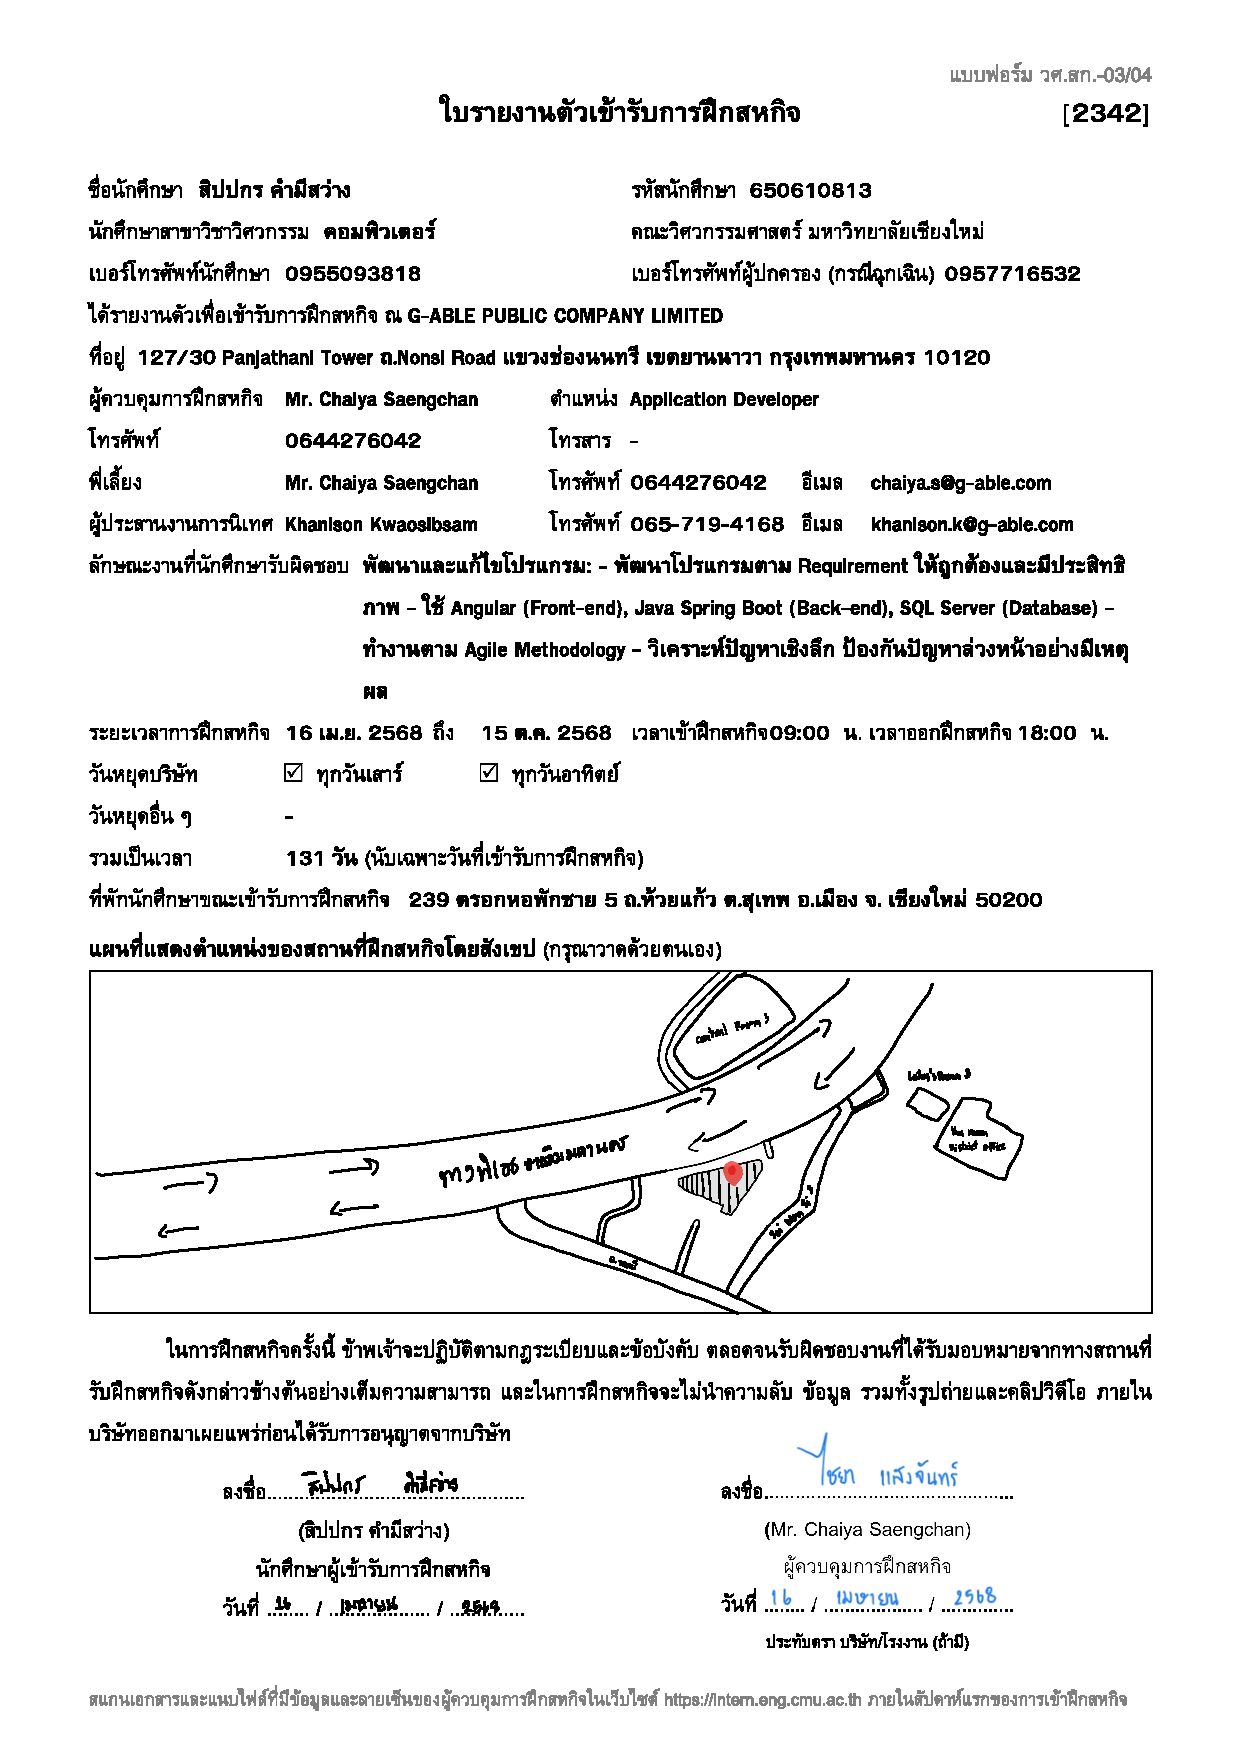
\includepdf[pages=-, scale=.8, pagecommand={\hypertarget{target:03-04}{},\label{page:03-04}}, nup=1x1, frame=false]{pdf/03-04_flat}
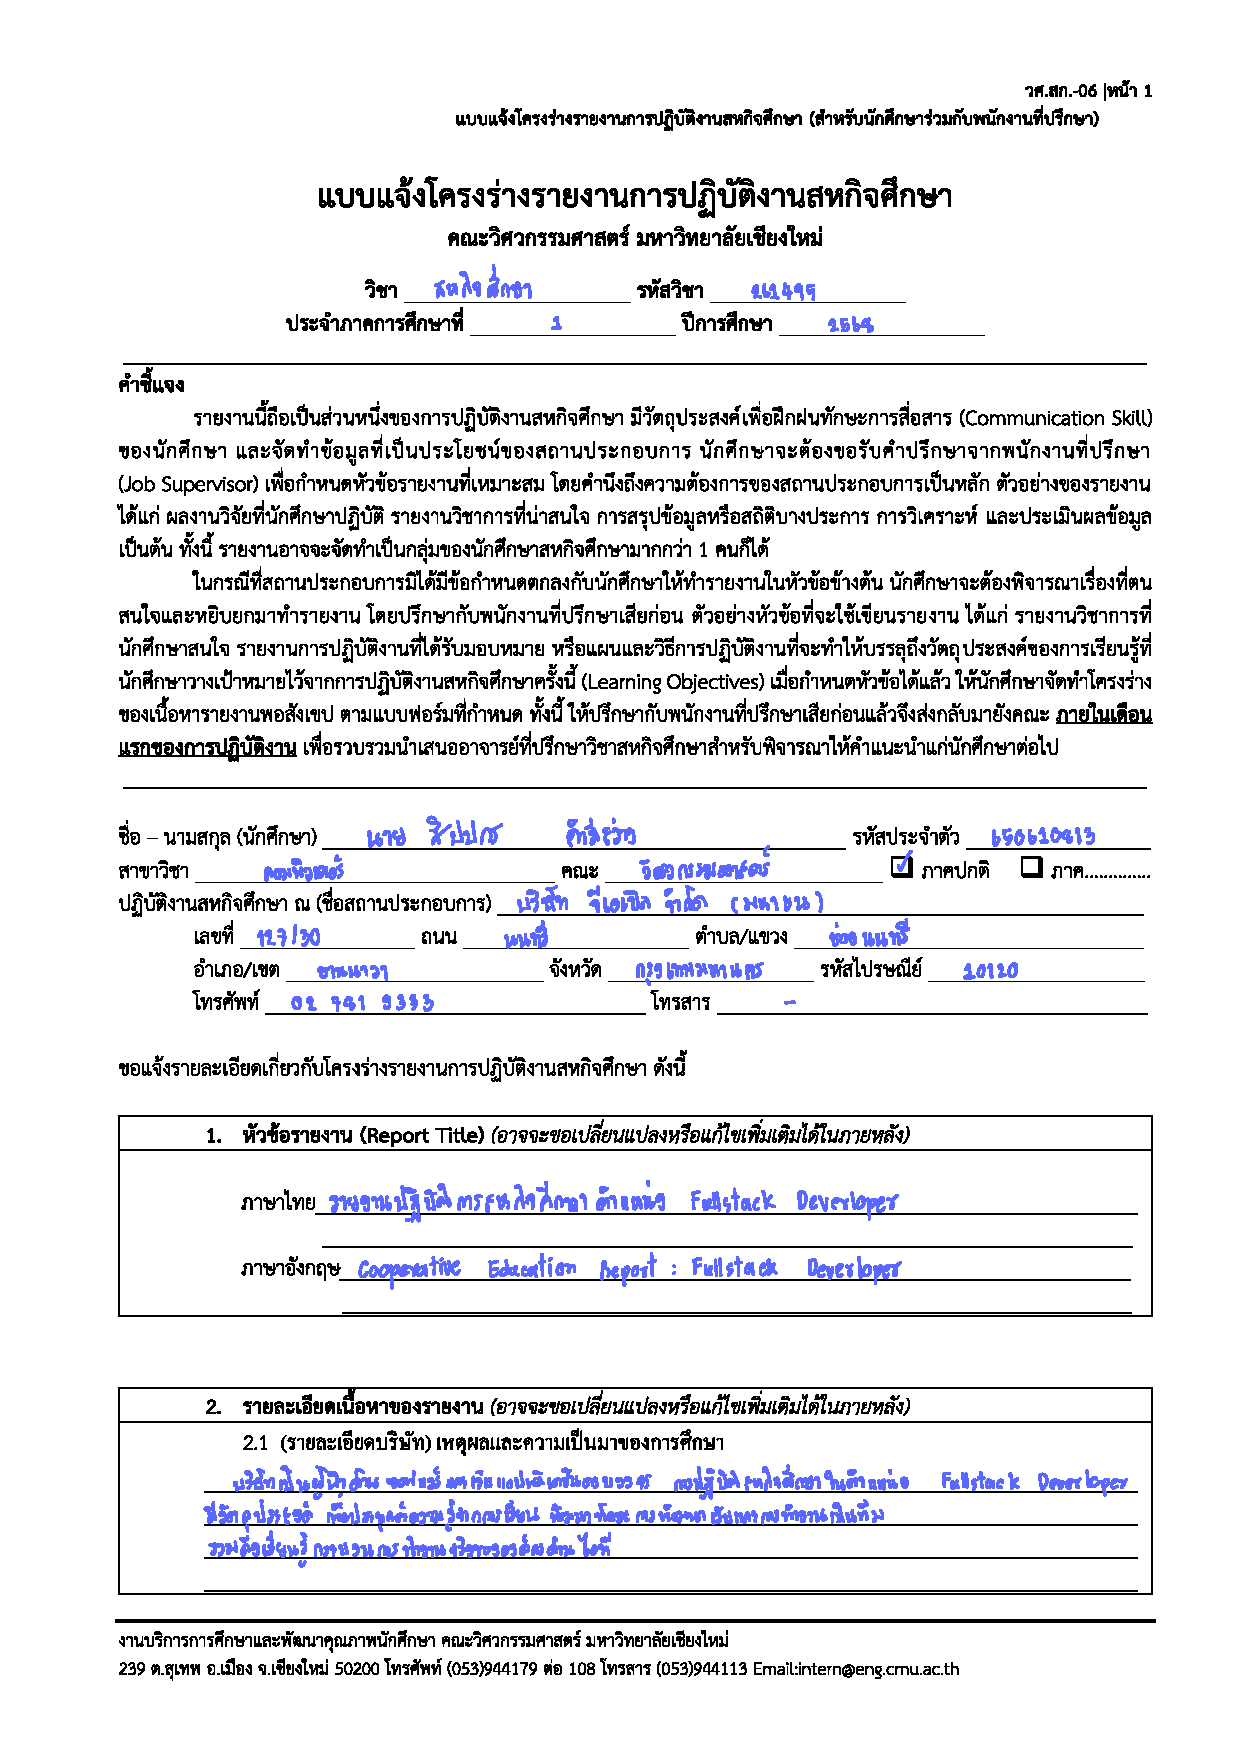
\includepdf[pages=-, scale=.8, pagecommand={\hypertarget{target:06}{},\label{page:06}}, nup=1x1, frame=false]{pdf/06_flat}
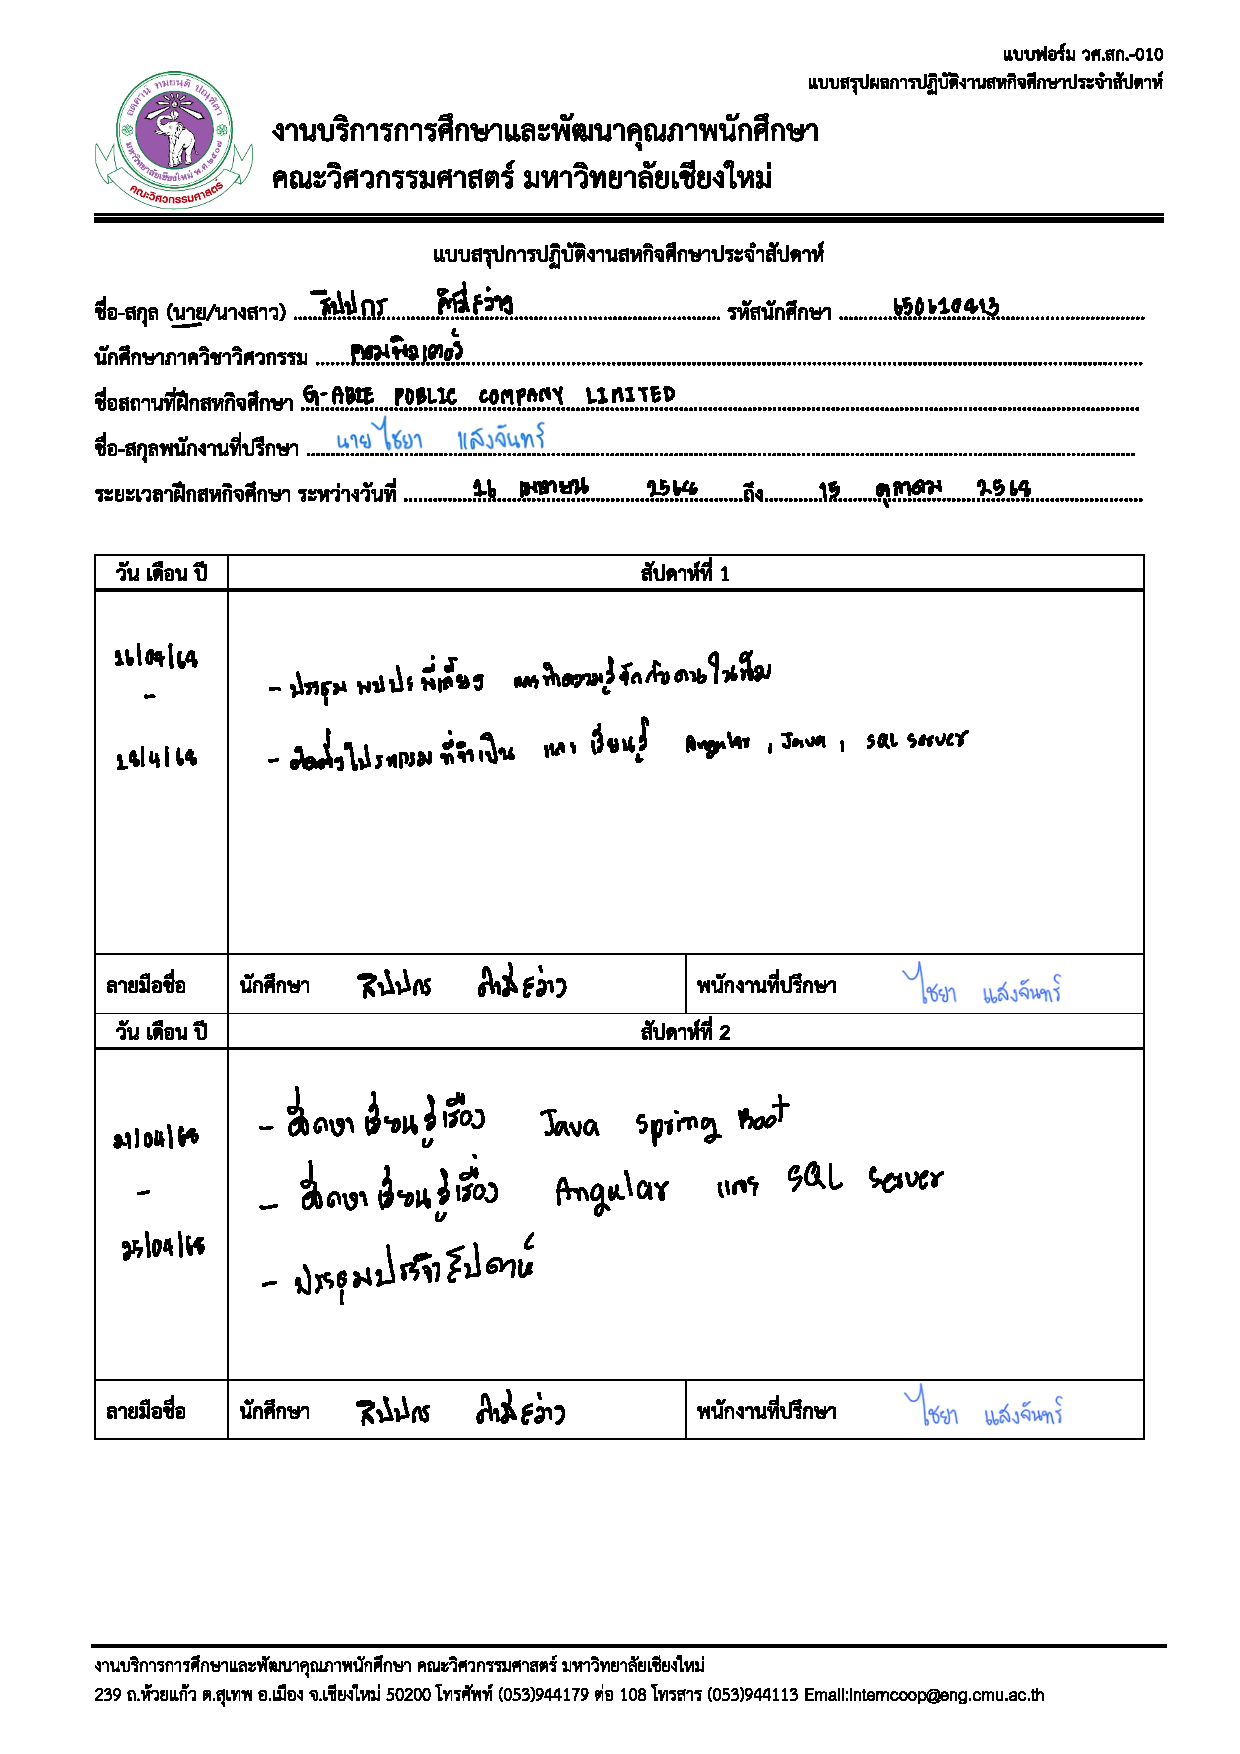
\includepdf[pages=-, scale=.8, pagecommand={\hypertarget{target:10}{},\label{page:10}}, nup=1x1, frame=false]{pdf/10_flat}
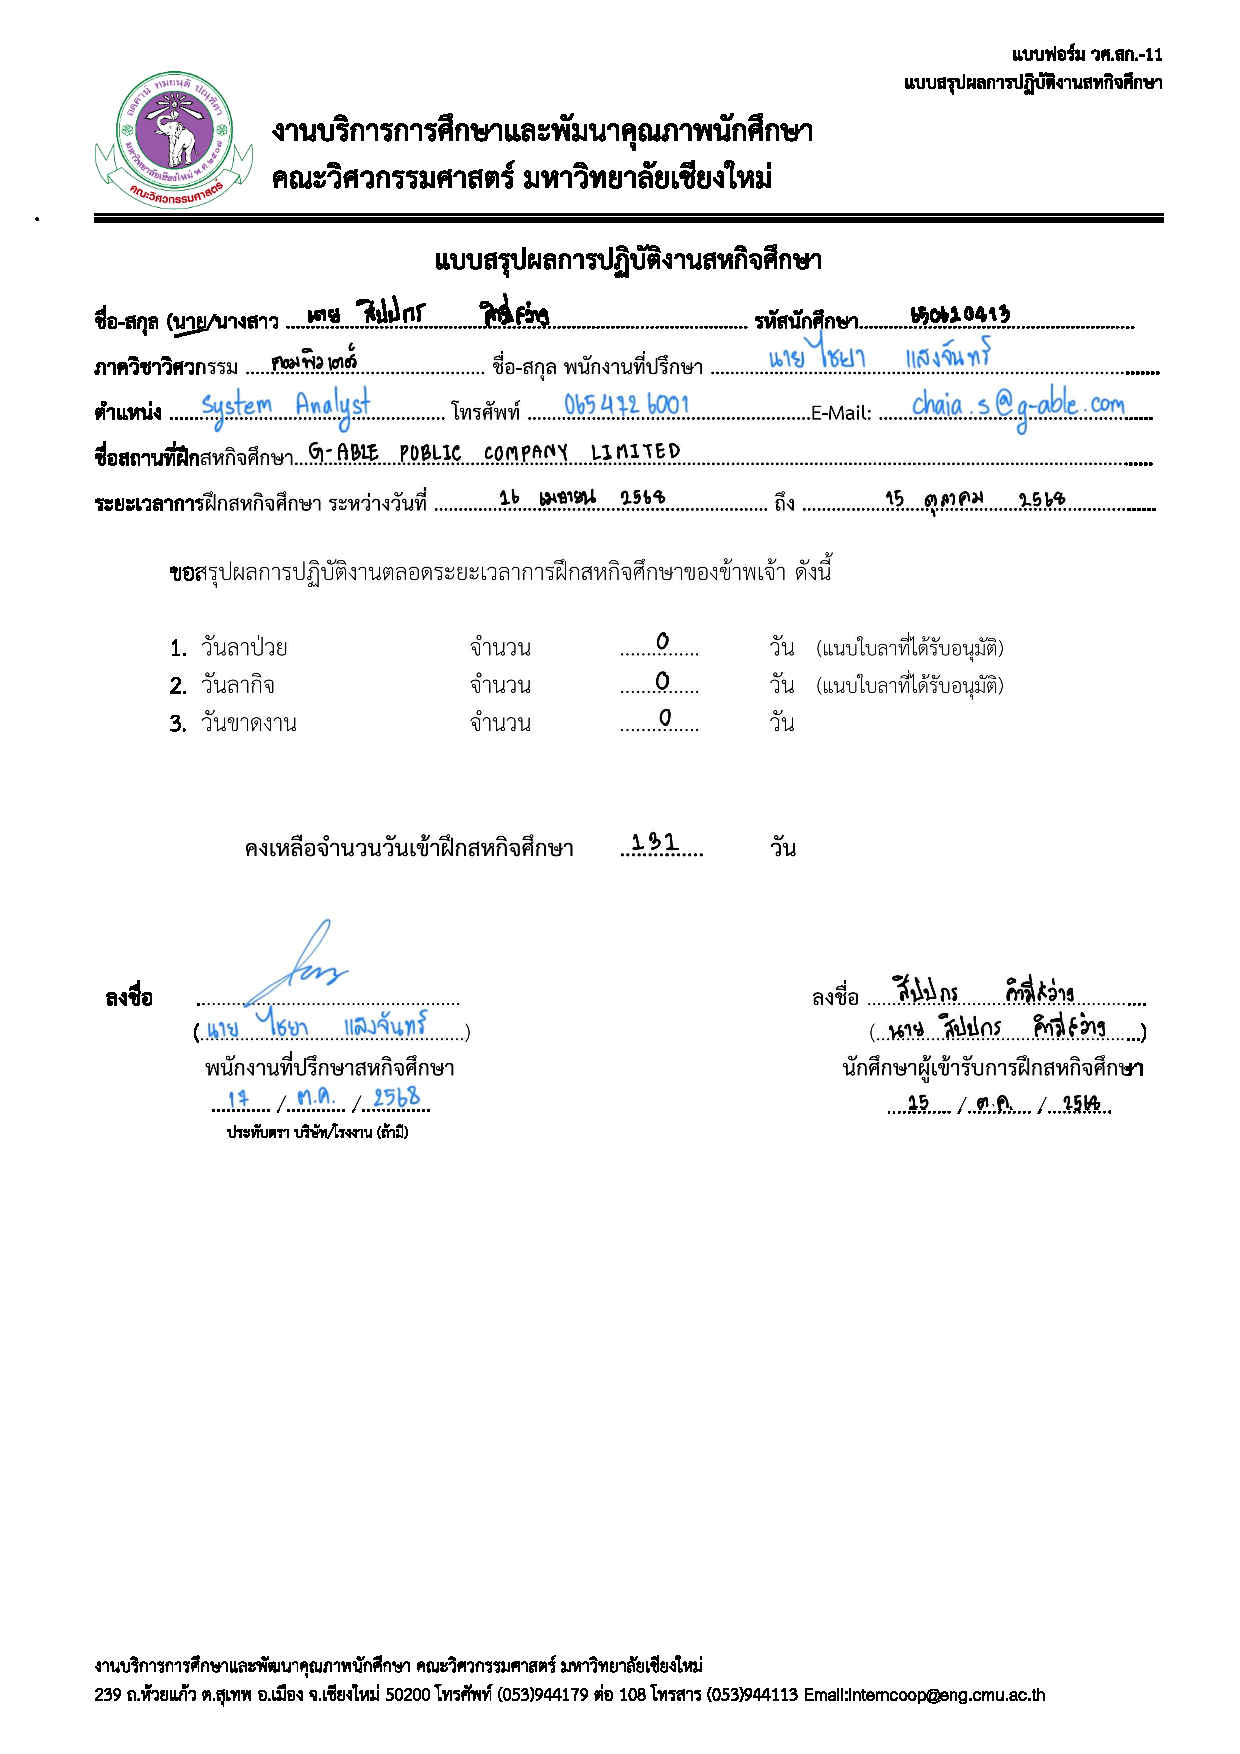
\includepdf[pages=-, scale=.8, pagecommand={\hypertarget{target:11}{},\label{page:11}}, nup=1x1, frame=false]{pdf/11_flat}

% ส่วนที่เกี่ยวข้อง
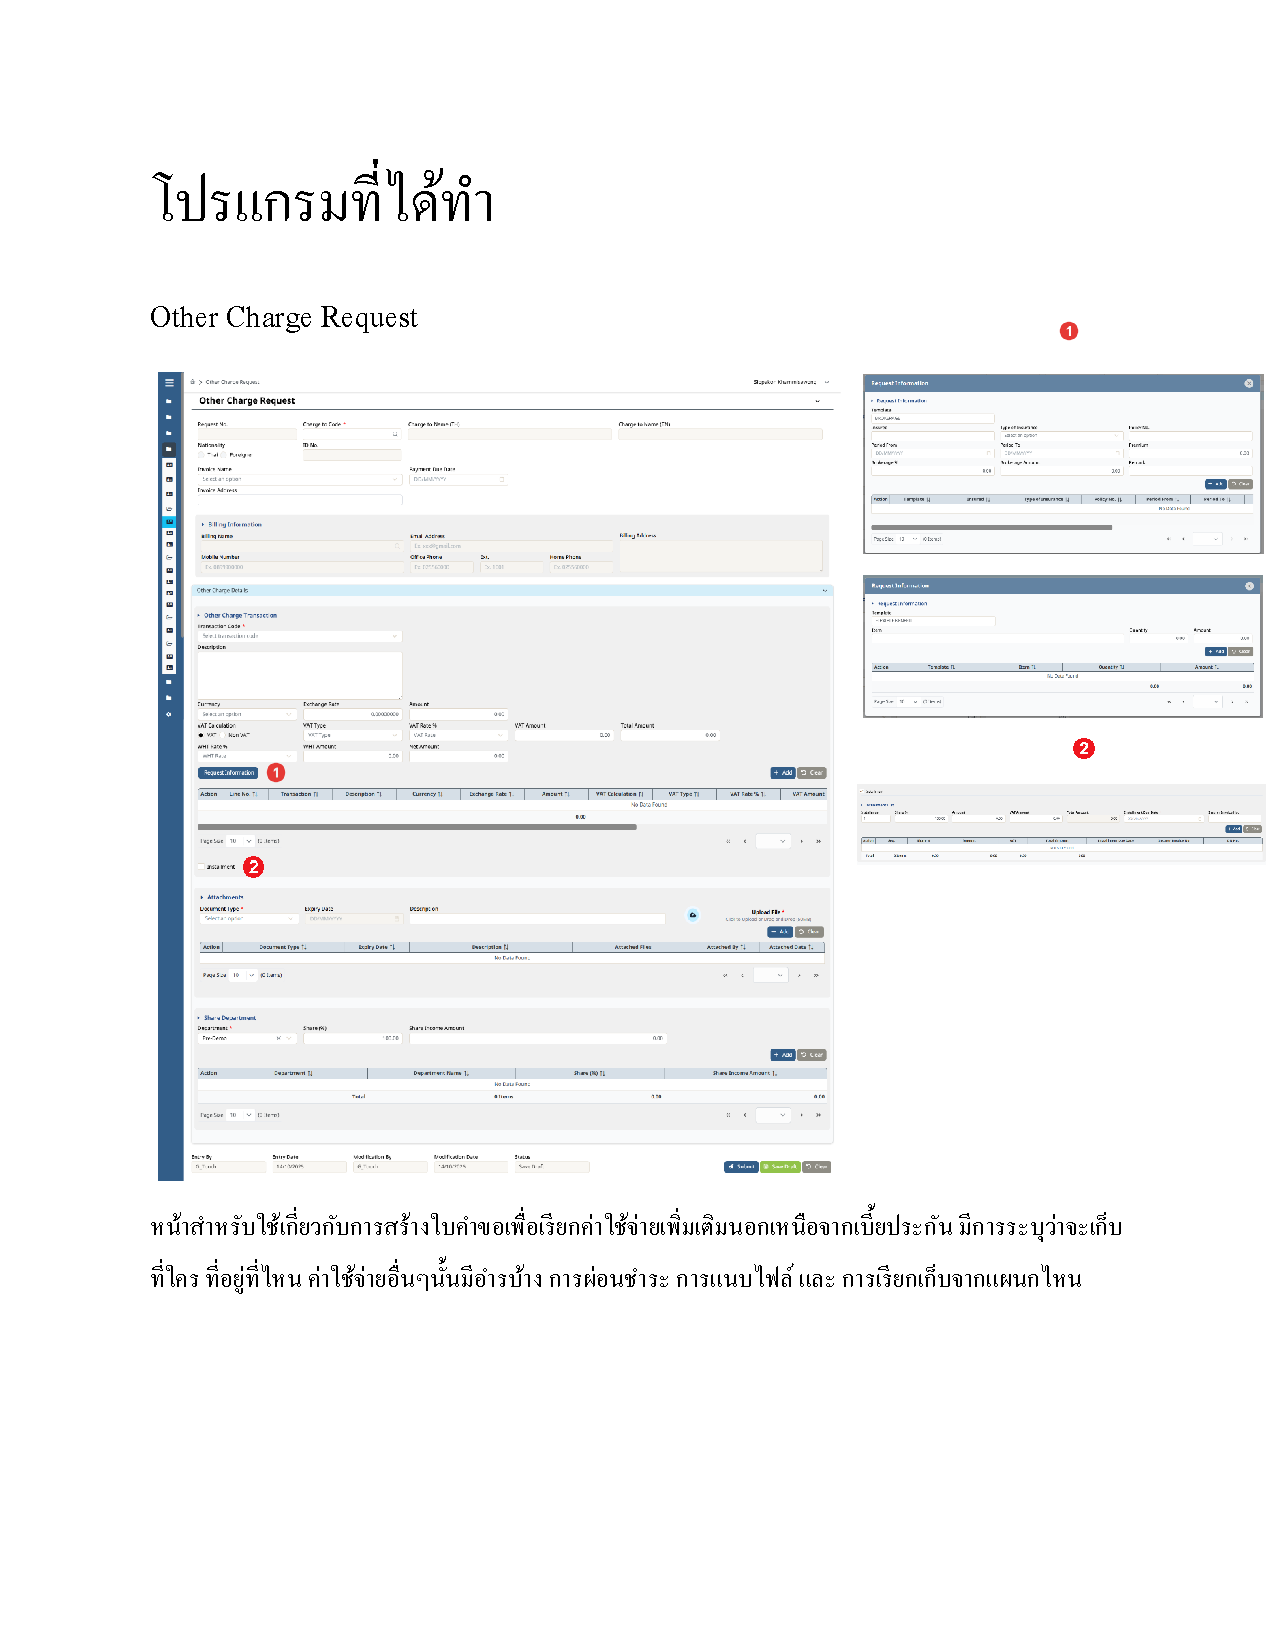
\includepdf[pages=-, scale=.8, pagecommand={\hypertarget{target:create}{},\label{page:create}}, nup=1x1, frame=false]{pdf/create}
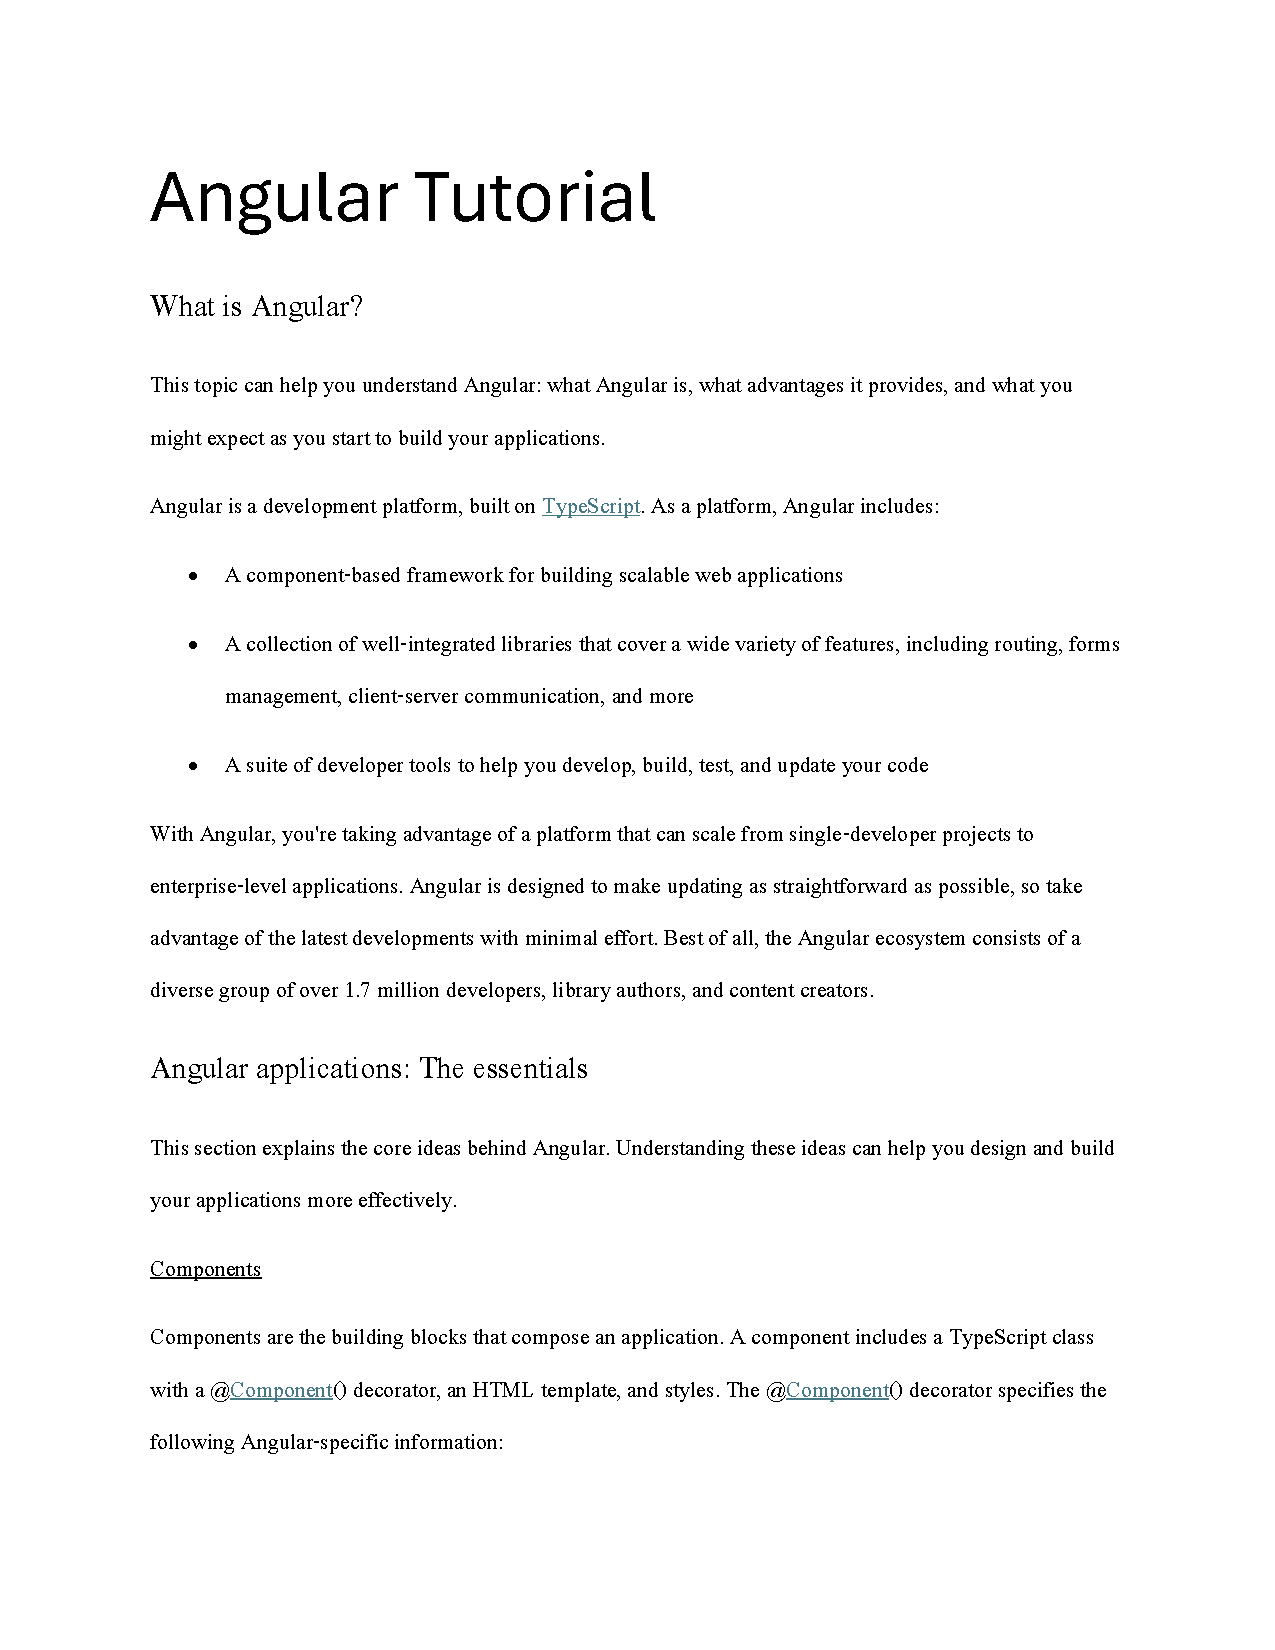
\includepdf[pages=-, scale=.8, pagecommand={\hypertarget{target:angular}{},\label{page:angular}}, nup=1x1, frame=false]{pdf/angular}
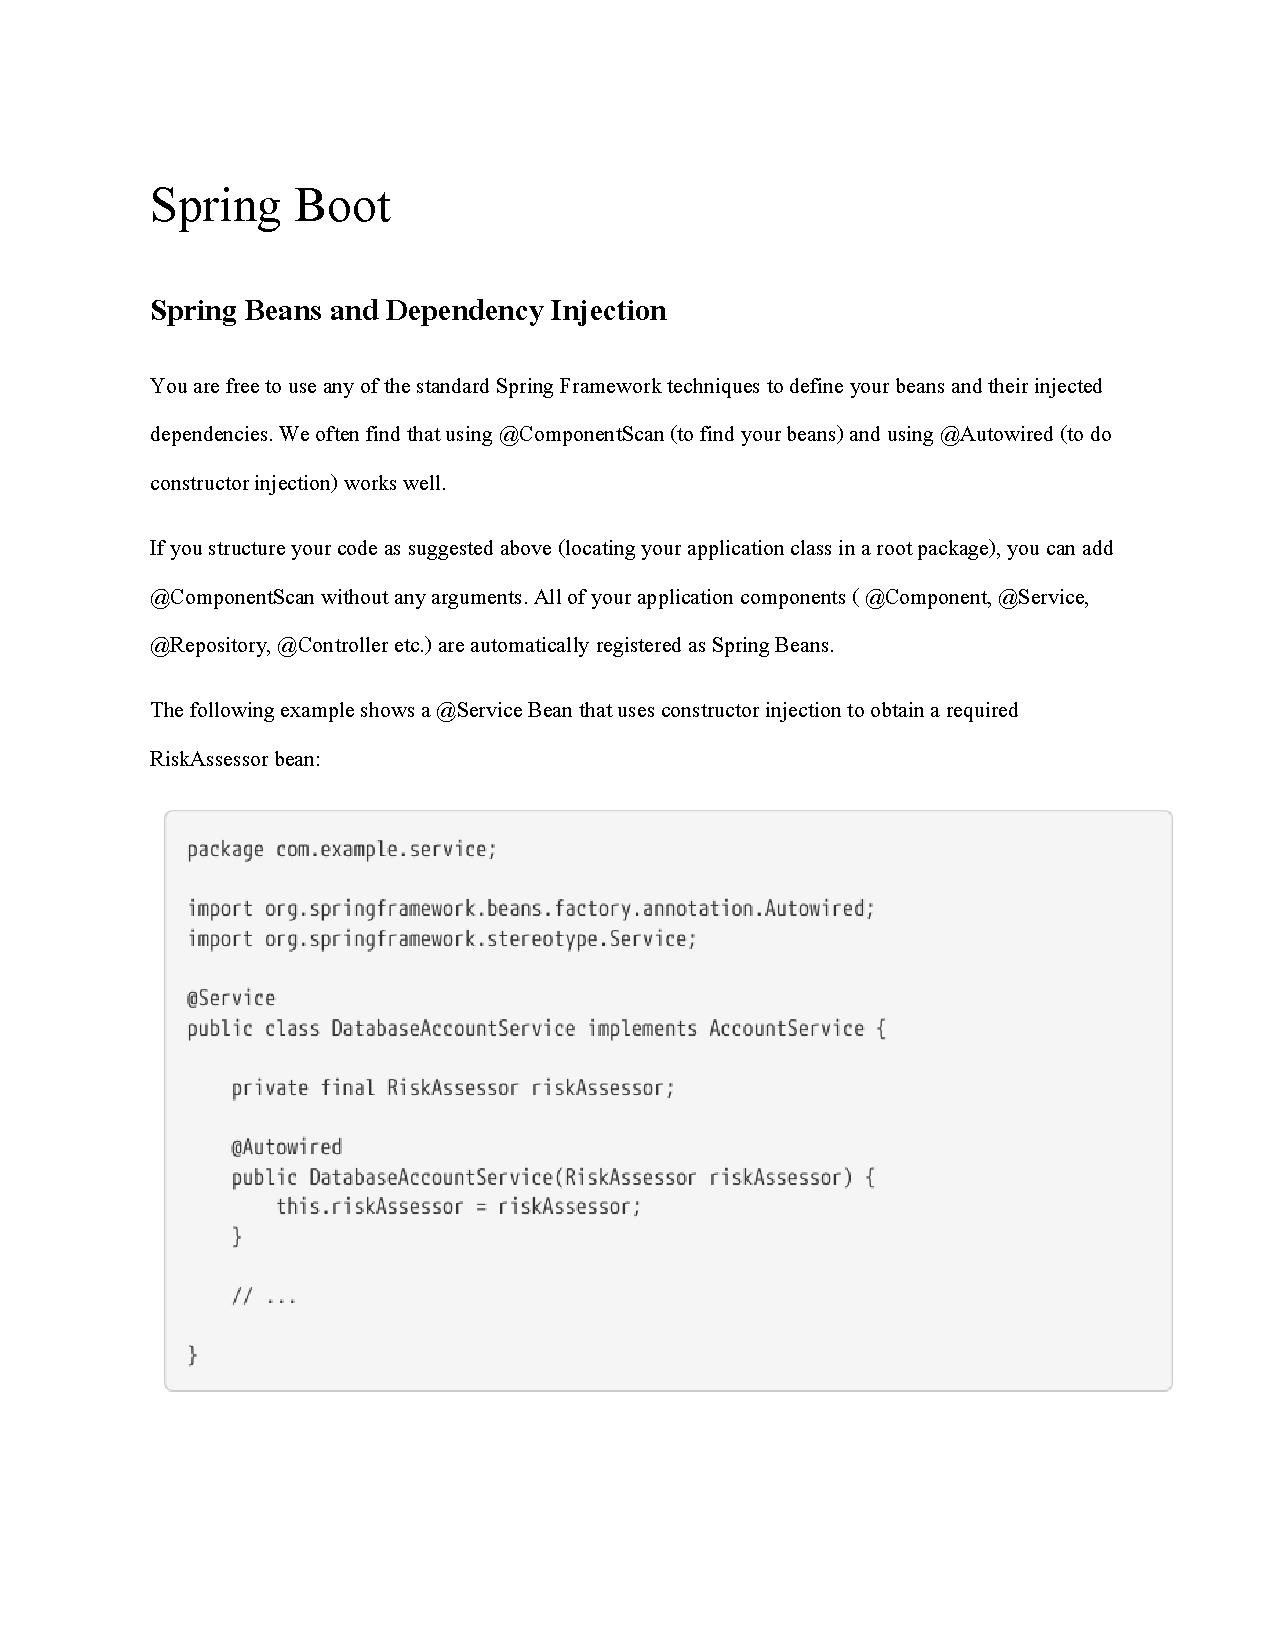
\includepdf[pages=-, scale=.8, pagecommand={\hypertarget{target:springboot}{},\label{page:springboot}}, nup=1x1, frame=false]{pdf/springboot}
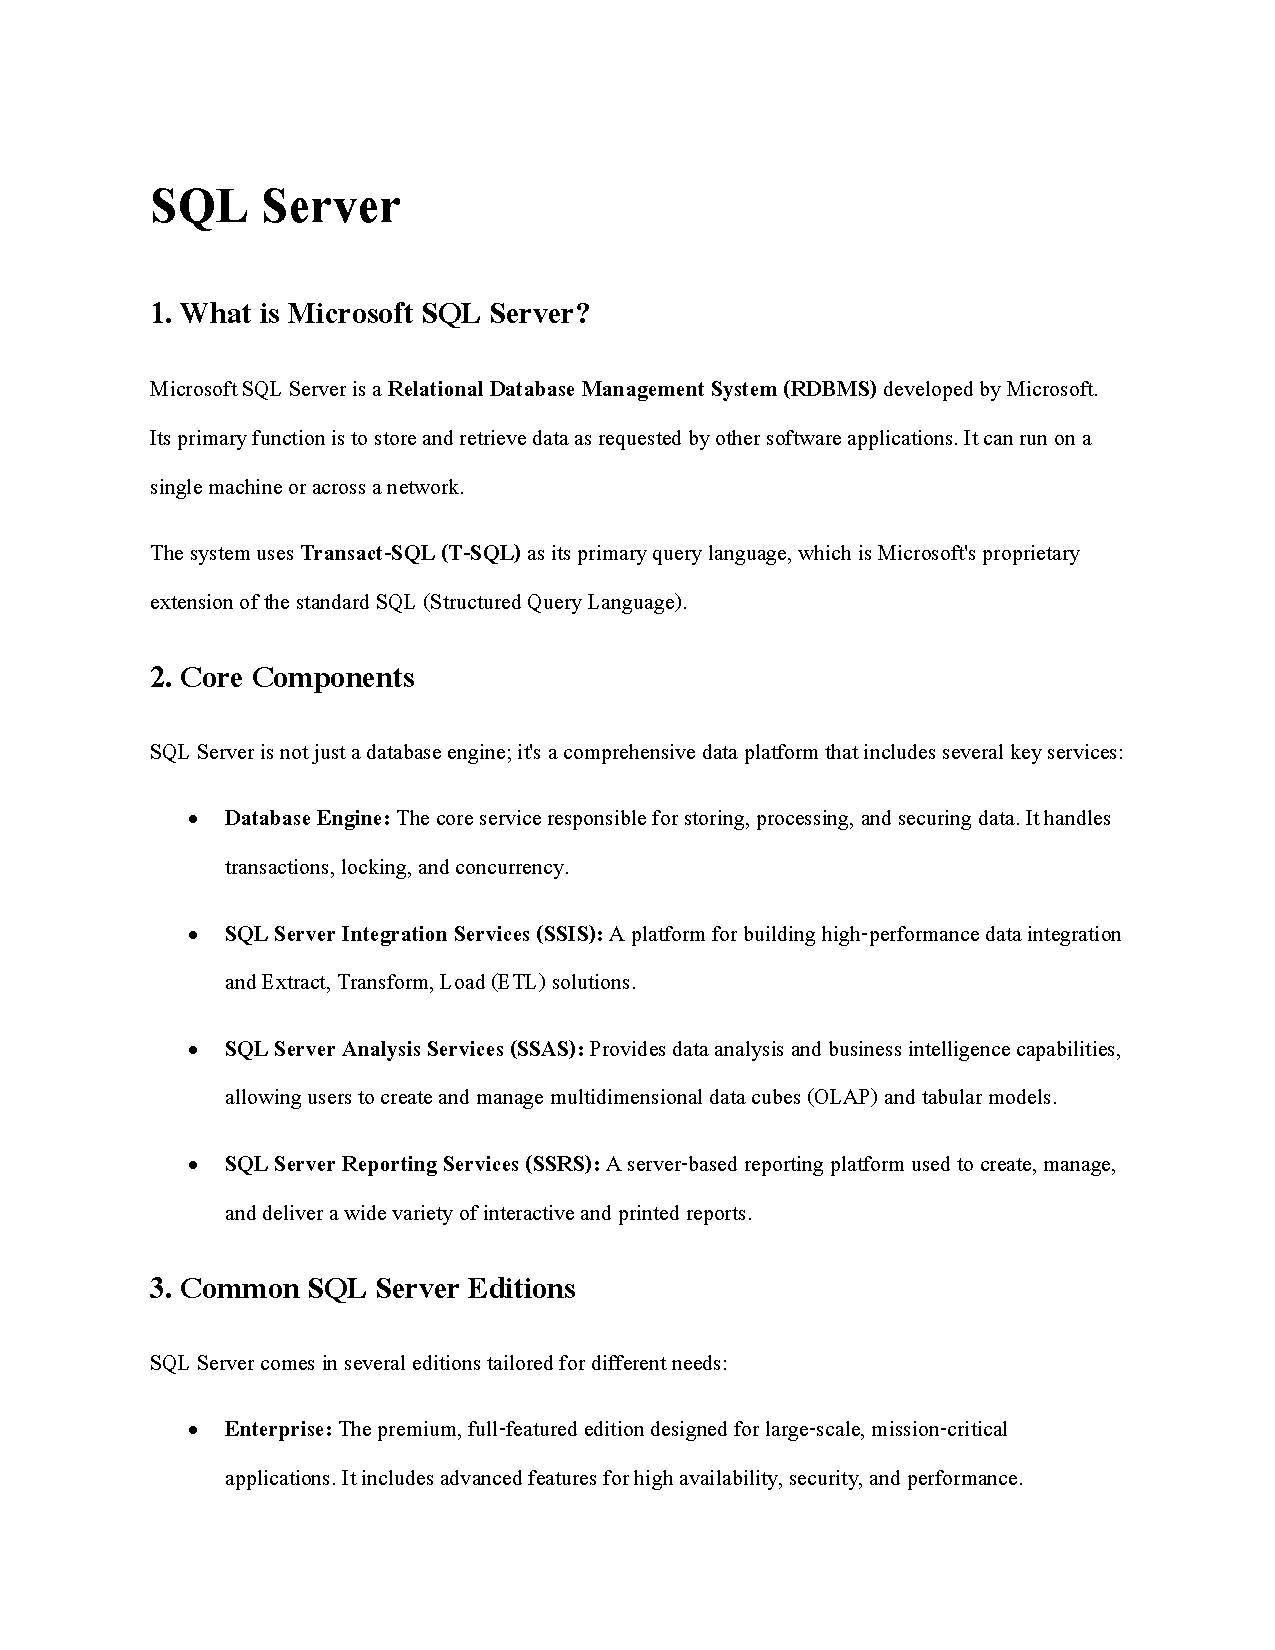
\includepdf[pages=-, scale=.8, pagecommand={\hypertarget{target:sqlserver}{},\label{page:sqlserver}}, nup=1x1, frame=false]{pdf/sqlserver}


%% Display glossary (optional) -- need glossary option.
\ifglossary\glossarypage\fi

%% Display index (optional) -- need idx option.
\ifindex\indexpage\fi

\fi % \ifproject
\end{document}
